\documentclass{article}
\usepackage{graphicx}
\usepackage{url}
\usepackage{amssymb}
\usepackage{amsmath}
\usepackage{hyperref}
\usepackage{verbatim}
\usepackage{natbib}

%\VignetteIndexEntry{Reading multiple tables of data}
%\VignettePackage{multitable}
%\VignetteDepends{multitable}
%\VignetteKeywords{data manipulation, ecology, multivariate, R}


%%%%R commands for running Sweave%%%%%%%
%%%%setwd("/users/stevenwalker/documents/multitable/multitable/vignettes/readingmultipletables/")
%%%%Sweave("/users/stevenwalker/documents/multitable/multitable/vignettes/readingmultipletables/readingmultipletables.Rnw")



\newcommand{\R}{{\sf R}}
\newcommand{\code}[1]{\texttt{#1}}
\title{Reading multiple tables of data into \R}
\author{SC Walker}

\newcounter{exercise}
\numberwithin{exercise}{section}
\newcommand{\exnumber}{\addtocounter{exercise}{1} \theexercise \thinspace}

\usepackage{Sweave}
\begin{document}
\maketitle
\tableofcontents

\begin{abstract}
This vignette introduces several methods for creating \code{data.list} objects in the \code{multitable} package.
\end{abstract}



\section{Introduction}

The \code{multitable} package works by organizing multiple-table data into special \R\ objects called \code{data.list}s.  If you do not have the \code{multitable} package, you can get it \href{https://r-forge.r-project.org/R/?group_id=1171}{here}.  Everything in this vignette assumes that this package is installed and loaded, for example with the \code{library} function,
\begin{Schunk}
\begin{Sinput}
> library(multitable)
\end{Sinput}
\end{Schunk}

There are many methods for converting multiple-table data into a \code{data.list}.  The methods largely differ based on the format of the data to be converted.  Table \ref{tab:functions} gives a list of functions that can be used to create \code{data.list} objects, and the \R\ objects that they take as input.  This vignette illustrates the use of several of these functions.

\begin{table}
\caption{Functions that generate \code{data.list} objects as output}
\begin{center}
\begin{tabular}{p{3cm}p{8cm}}
\hline
Function & Input objects \\
\hline
%\code{as.data.list} & either a \code{vector}; \code{matrix}; \code{array}; \code{data.frame}; \code{list}; or a \code{list} of such objects \\
\code{data.list} & a number of \code{vector}s; \code{matrix}es; \code{array}s; \code{data.frame}s; and \code{list}s \\
\code{dlcast} & a \code{list} of long-format \code{data.frame}s \\
\code{read.multitable} & character \code{vector} giving filenames of long-format text files \\
\code{read.multicsv} & character \code{vector} giving filenames of long-format comma-separated text files \\
\code{read.multidelim} & character \code{vector} giving filenames of long-format tab-delimited text files \\
\code{read.fourthcorner} & three character strings giving filenames of the data tables that define a fourth-corner problem \\
\hline
\end{tabular}
\end{center}
\label{tab:functions}
\end{table}

%Here we organize this vignette by considering ?? approaches for doing so.  If your data are in standard `fourth-corner' format and would like to get going as quickly as possible, see Section ??.  If you would like a good general-purpose step-by-step method that follows many of the `best-practices' often recommended in data management, then I recommend Section ??.  This section covers recommendations on how to format your data in Excel / text files, right up to the commands required to read these files into \R.  If you would like to understand some of the details behind these `best-practices' see Section ??.  And if you do not appreciate being told how to get your data into standard \R\ objects (e.g. \code{data.frame}s; \code{matrix}es), and would like to simply combine such objects into a \code{data.list} then see Section ??.

\section{Reading from text files directly into a \code{data.list}}

\subsection{Reading fourth corner data}

Figure \ref{fig:spreadsheetfc} \begin{figure}
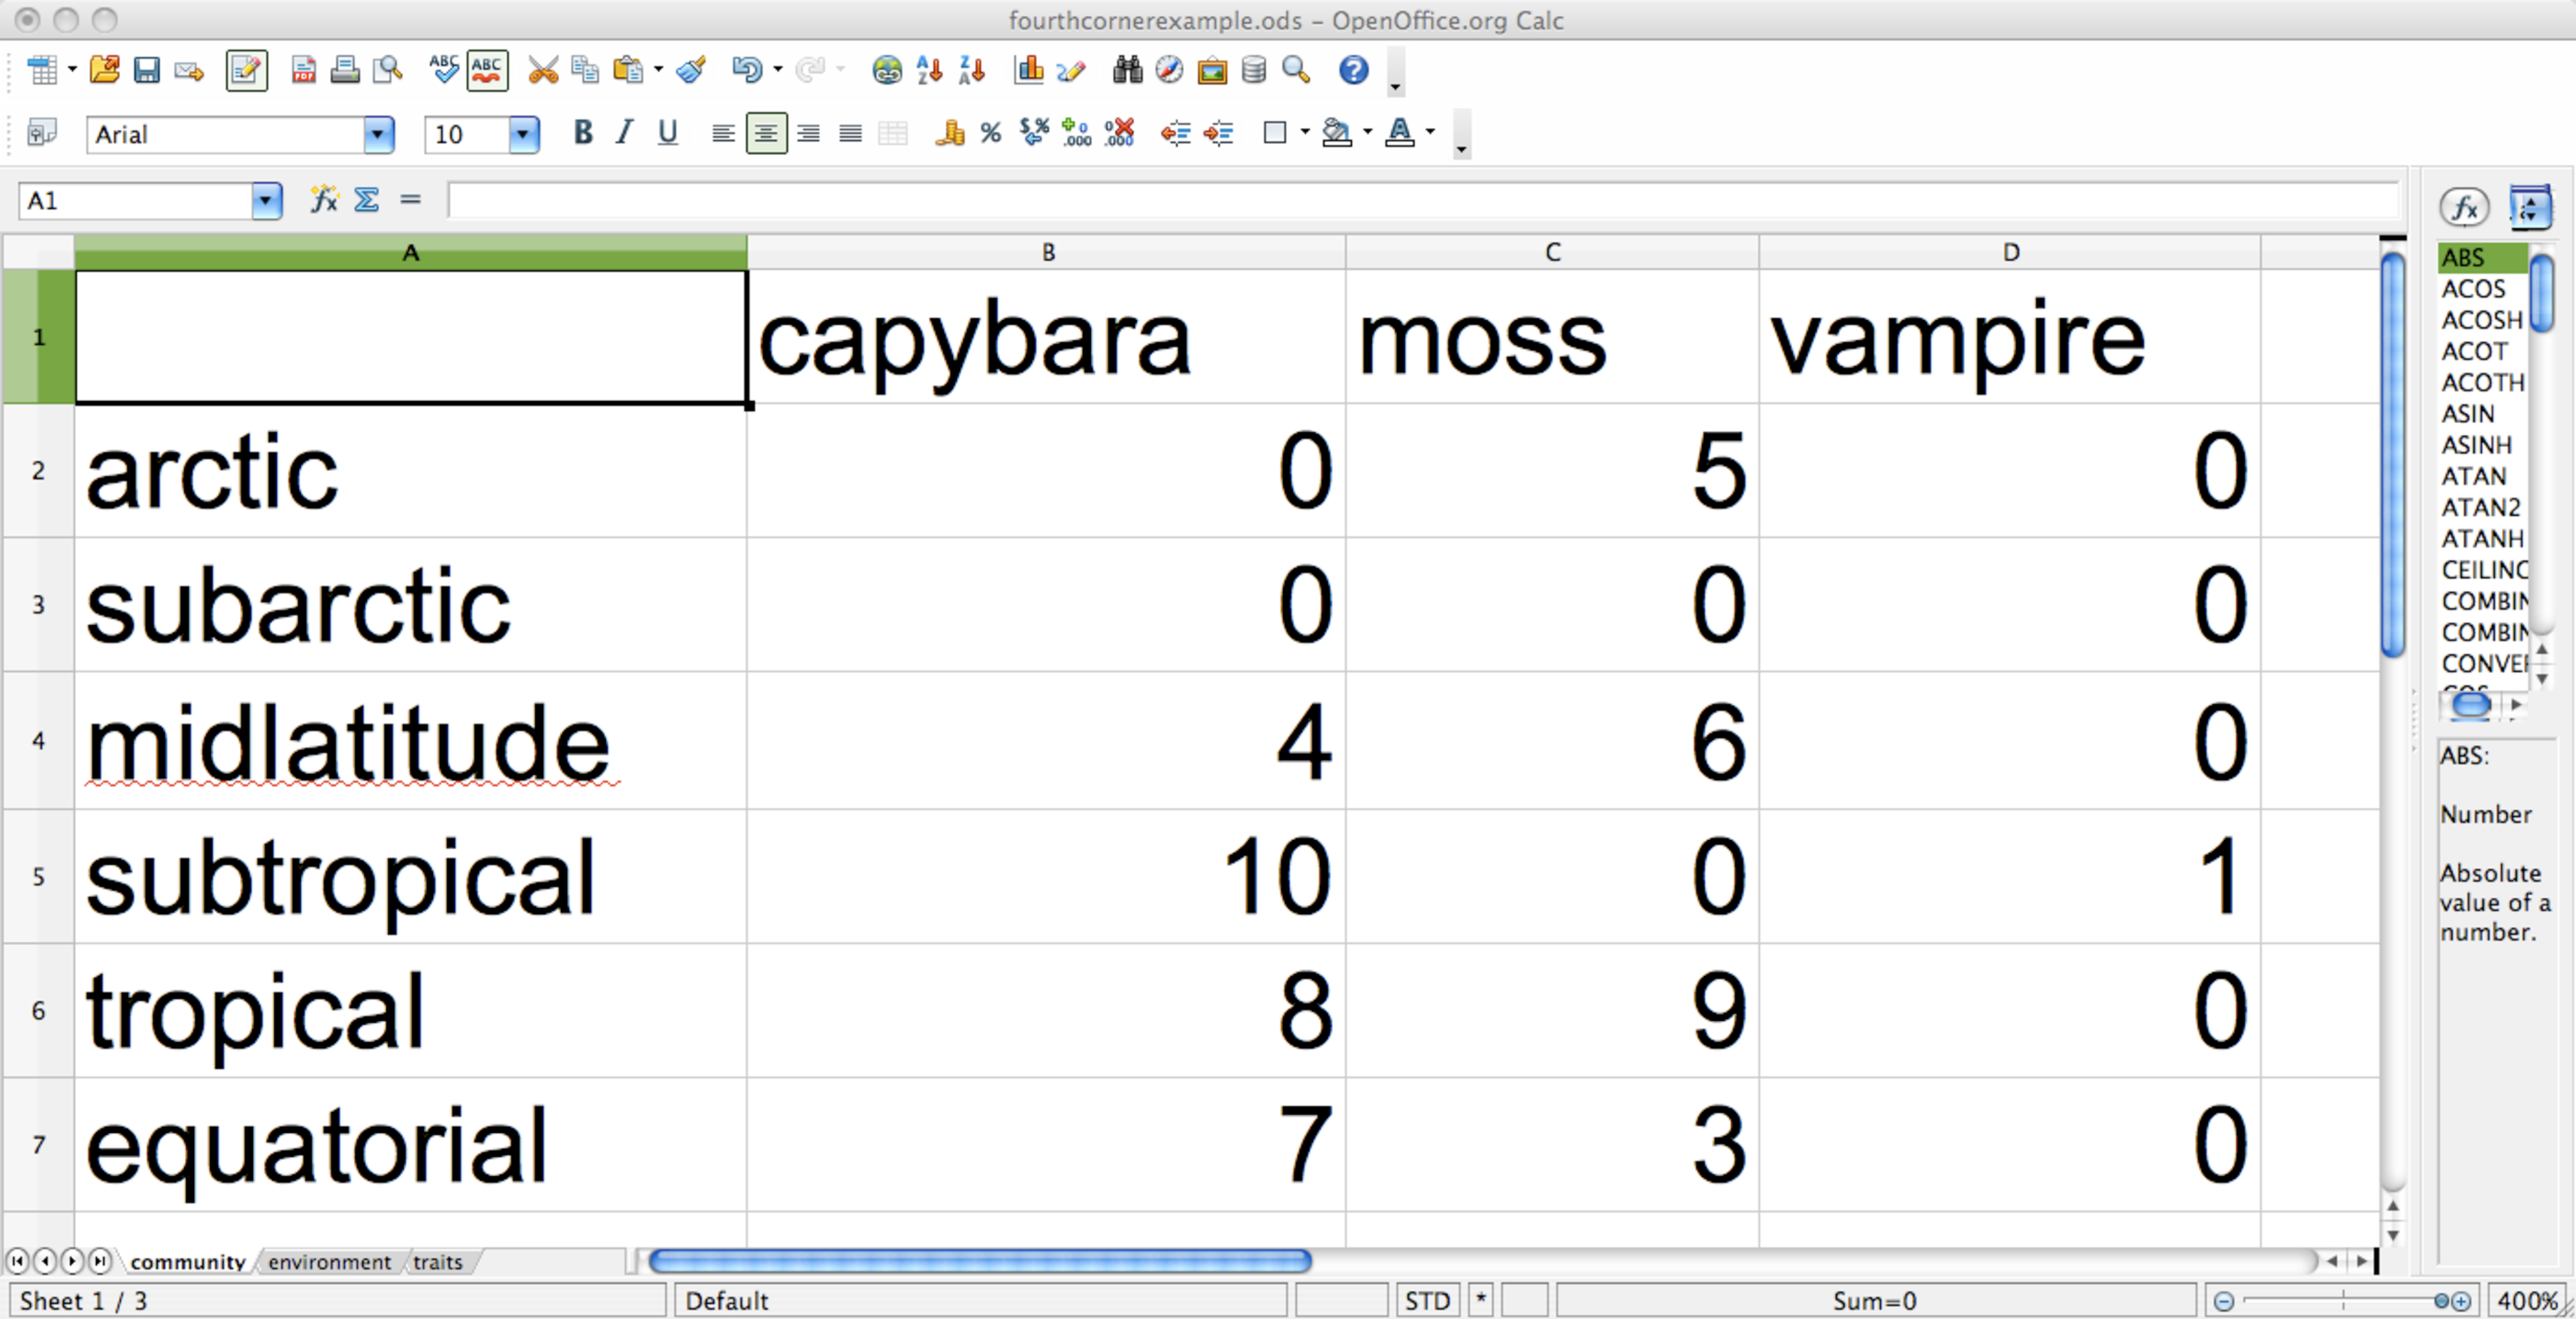
\includegraphics{./readingmultipletables/community.pdf}
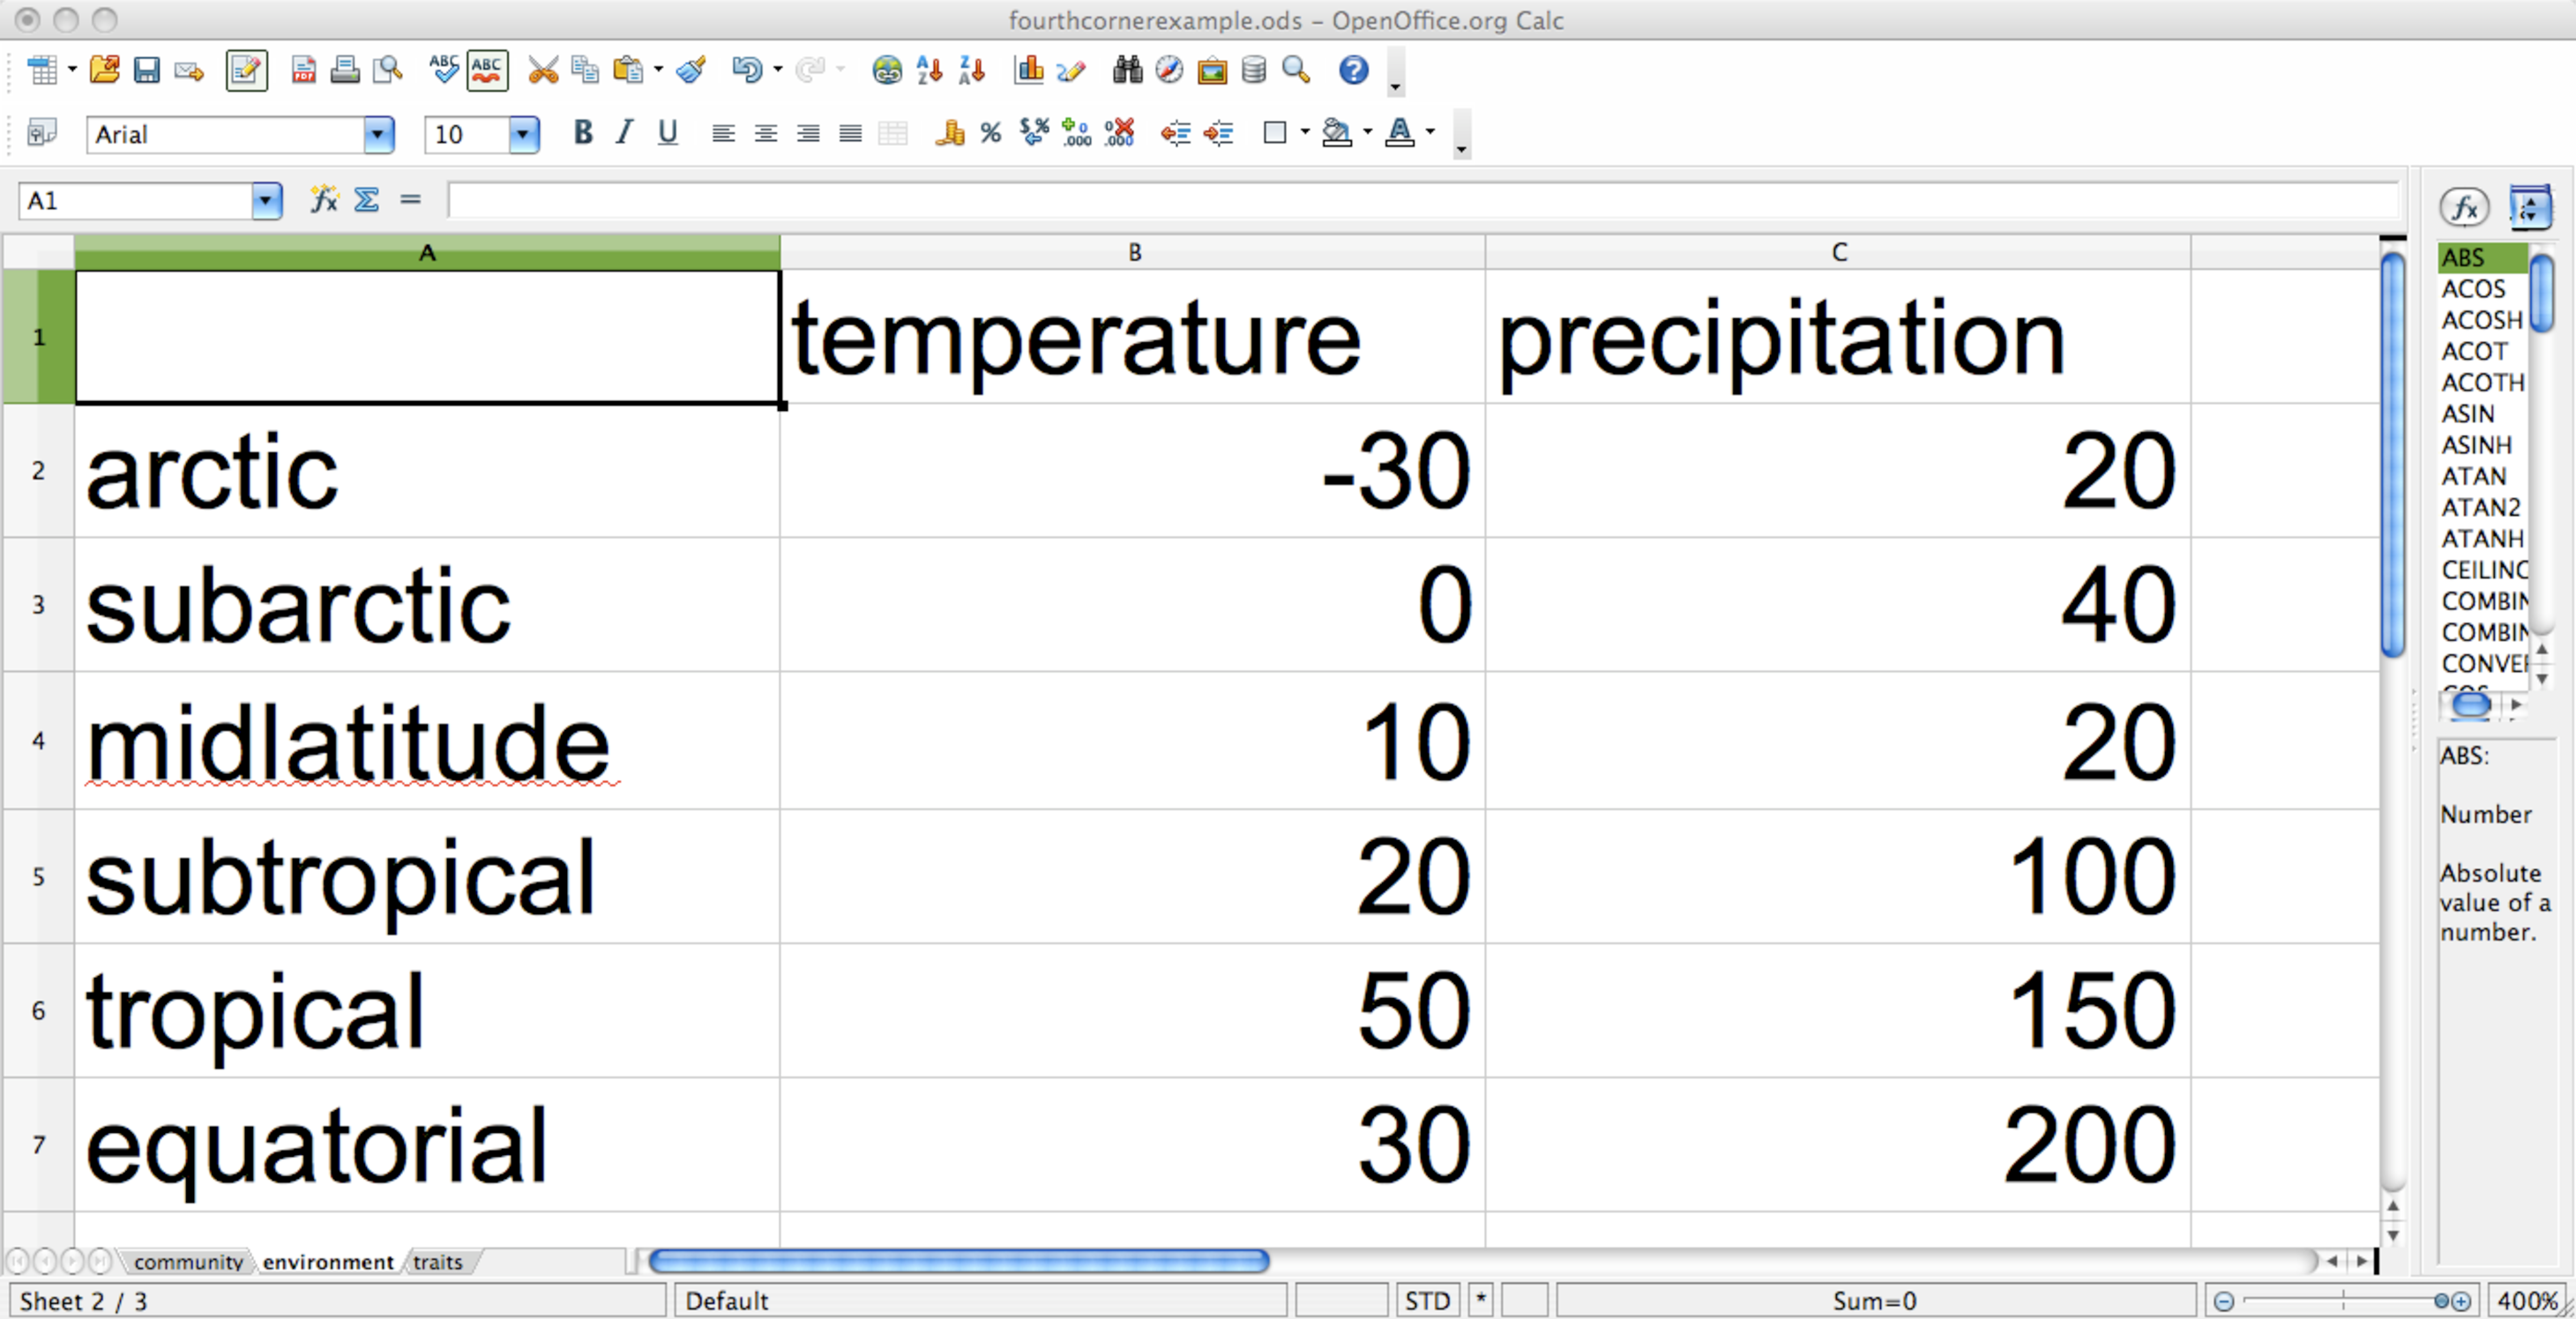
\includegraphics{./readingmultipletables/environment.pdf}
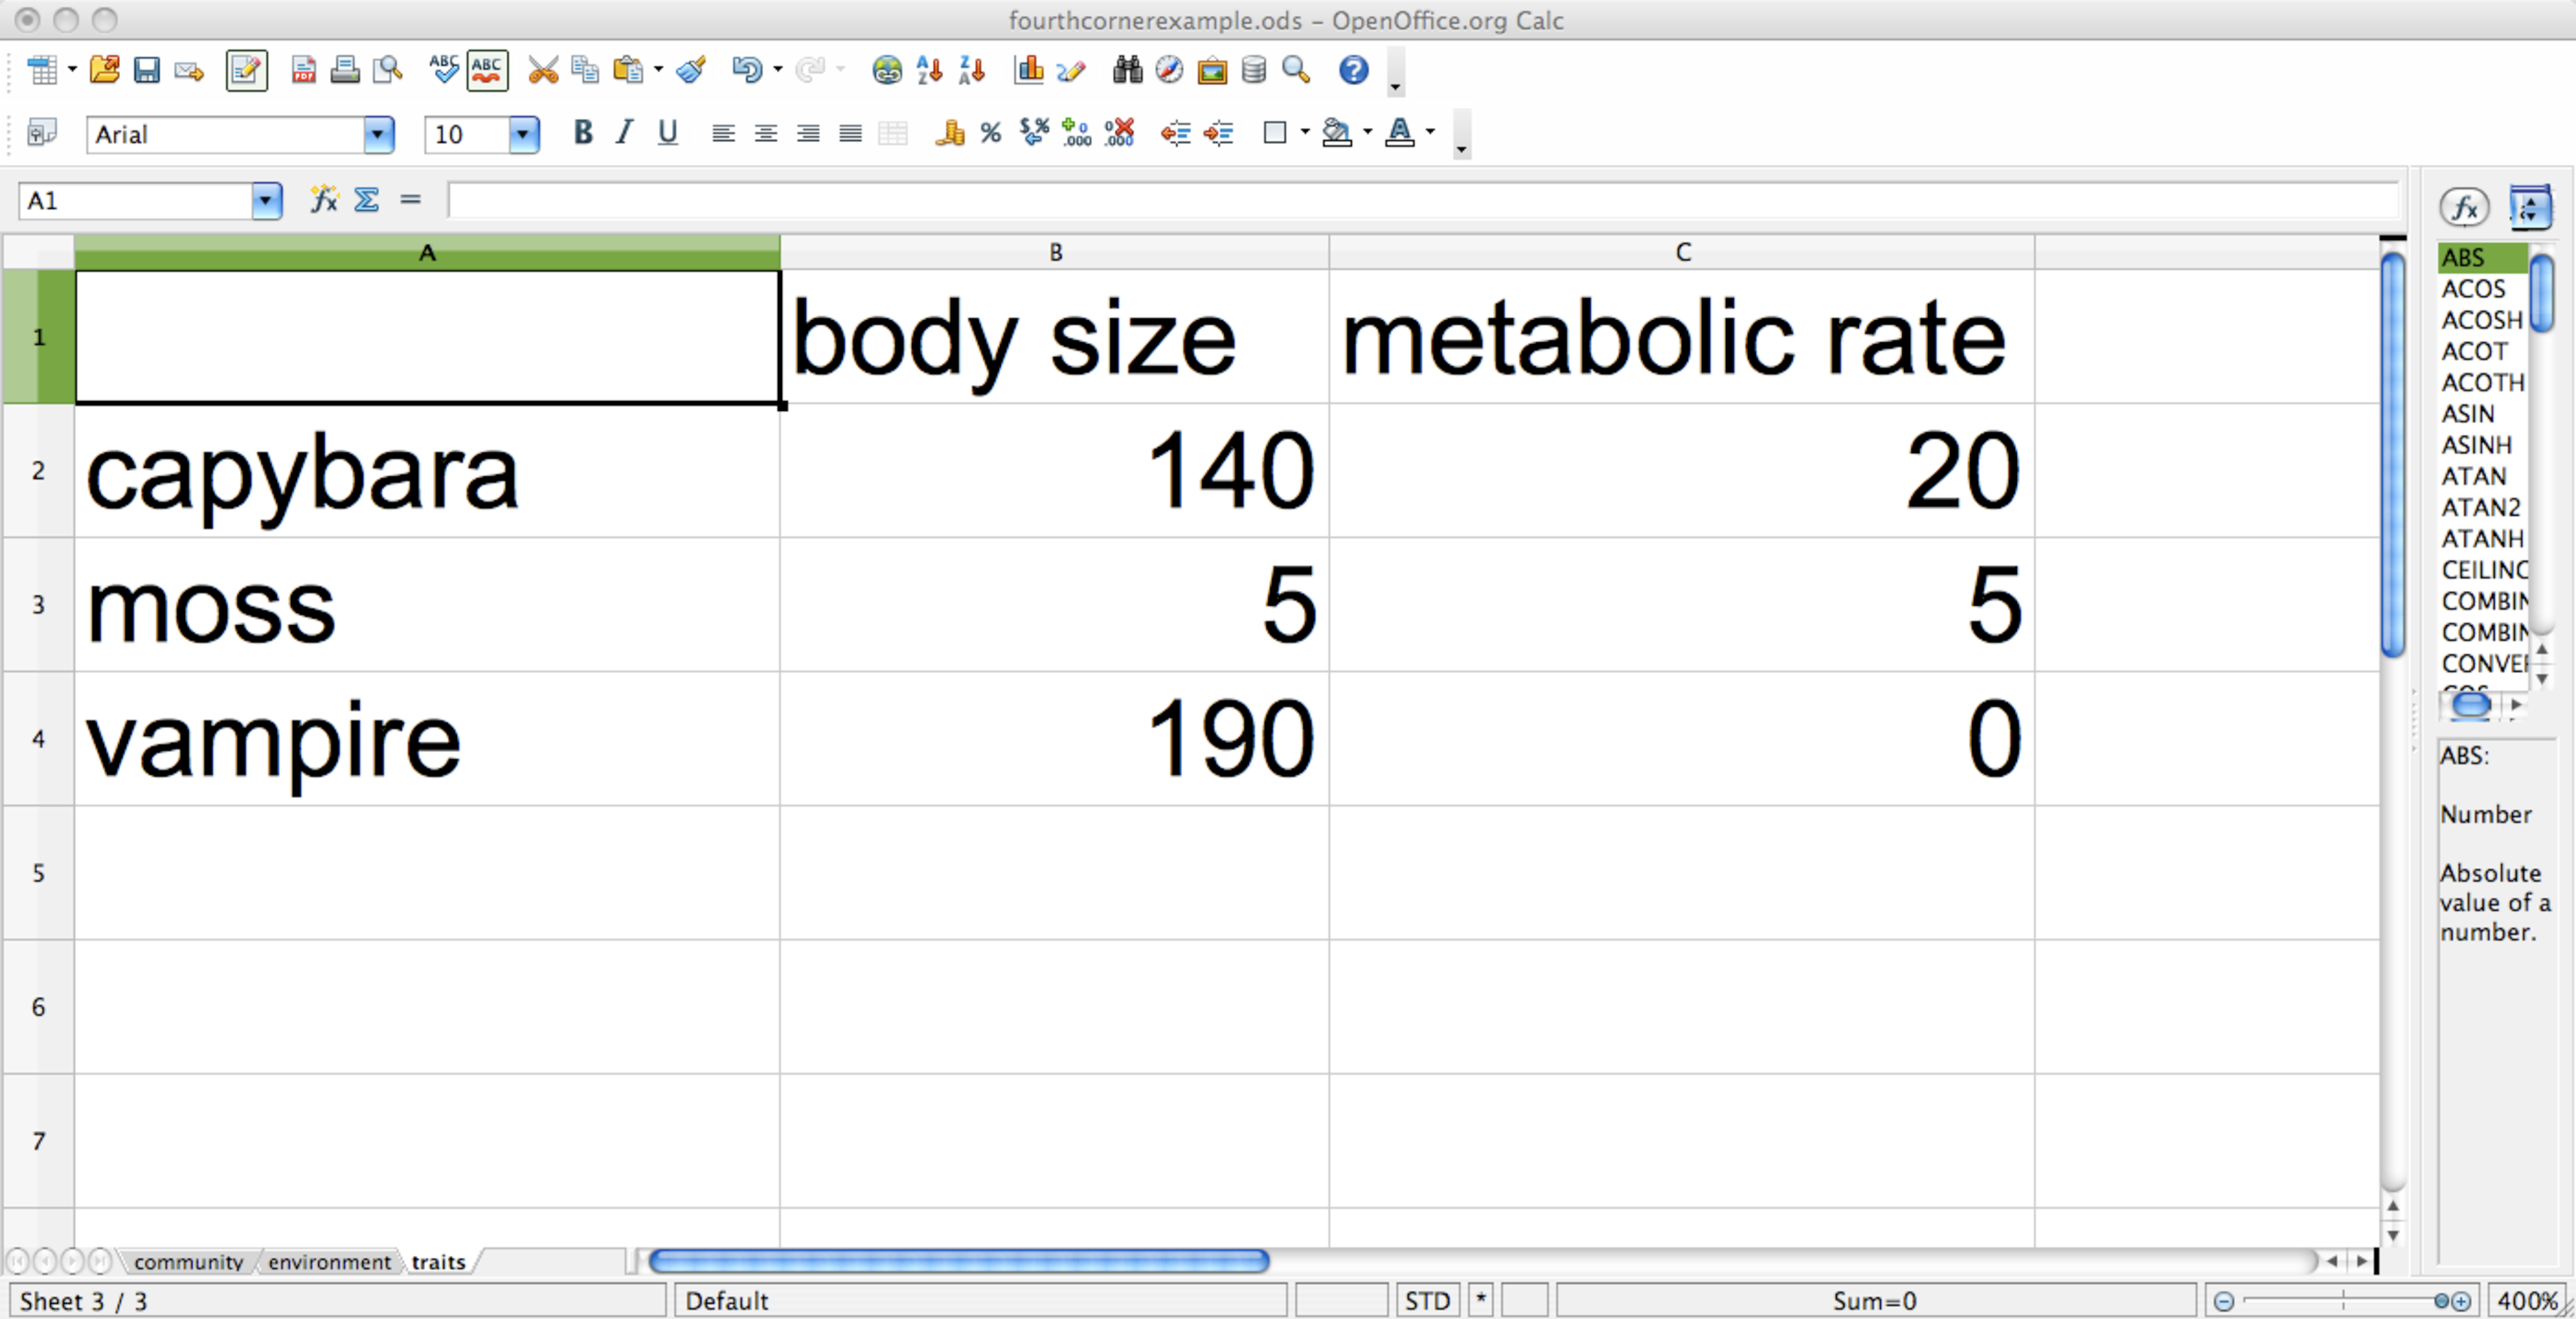
\includegraphics{./readingmultipletables/traits.pdf}
\caption{Fictitious fourth-corner data set.}
\label{fig:spreadsheetfc}
\end{figure}shows three spreadsheets containing the data for a simple fourth-corner problem \citep{LegendreEtAl1997}.  The first sheet gives species abundance data for three species (capybara; moss; vampire) at six sites (arctic; subarctic; midlatitude; subtropical; tropical; equatorial).  The second and third sheets give two environmental variables (temperature; precipitation) at each site and two traits (body size; metabolic rate) for each species.  We are going to convert these spreadsheets into an \R\ object that contains all of these variables, relating them along their shared dimensions.

Although it is possible to load spreadsheets directly into \R, it is usually better to first convert them into text files---I follow this \href{http://cran.r-project.org/doc/manuals/R-data.html#Reading-Excel-spreadsheets}{standard advice}.  To convert to a text file, open a spreadsheet, select \code{save as} from a menu, and choose a text file format (e.g. comma separated .csv file).

Once each of these three data tables is stored as a text file, then one line of \R\ code will read them all into a \code{data.list} object using the \code{read.fourthcorner} function in the \code{multitable} package,
\begin{Schunk}
\begin{Sinput}
> setwd("./readingmultipletables/")
> fc <- read.fourthcorner(
   "community.csv",
   "environment.csv",
   "traits.csv",
   sep=",",header=TRUE,row.names=1)
\end{Sinput}
\end{Schunk}
Note that this line assumes that the files are in the working directory.  If this is not true, then include the path in the string just as you would do with \code{read.table} or \code{read.csv}.  Alternatively, the \code{file.choose} function could be used as follows,
\begin{Schunk}
\begin{Sinput}
> fc <- read.fourthcorner(
   file.choose(),
   file.choose(),
   file.choose(),
   sep=",",header=TRUE,row.names=1)
\end{Sinput}
\end{Schunk}
to invoke an interactive menu for selecting the appropriate files.  The \code{header=TRUE} argument indicates that the first line in each file gives the names of the columns and \code{row.names=1} indicates that the first column in each file gives the names of the rows.  The \code{fc} object looks like this,
\begin{Schunk}
\begin{Sinput}
> fc
\end{Sinput}
\begin{Soutput}
abundance:
---------
            capybara moss vampire
arctic             0    5       0
subarctic          0    0       0
midlatitude        4    6       0
subtropical       10    0       1
tropical           8    9       0
equatorial         7    3       0
Replicated along:  || sites || species || 


temperature:
-----------
     arctic   subarctic midlatitude subtropical    tropical 
        -30           0          10          20          50 
 equatorial 
         30 
Replicated along:  || sites || 


precipitation:
-------------
     arctic   subarctic midlatitude subtropical    tropical 
         20          40          20         100         150 
 equatorial 
        200 
Replicated along:  || sites || 


body.size:
---------
capybara     moss  vampire 
     140        5      190 
Replicated along:  || species || 


metabolic.rate:
--------------
capybara     moss  vampire 
      20        5        0 
Replicated along:  || species || 


REPLICATION DIMENSIONS: 
  sites species 
      6       3 
\end{Soutput}
\end{Schunk}
and can be passed to various \R\ functions such as,
\begin{Schunk}
\begin{Sinput}
> glm(
   abundance~(temperature+precipitation)*(body.size+metabolic.rate),
   family=poisson,data=fc)
\end{Sinput}
\begin{Soutput}
Call:  glm(formula = abundance ~ (temperature + precipitation) * (body.size + 
    metabolic.rate), family = poisson, data = fc)

Coefficients:
                 (Intercept)                   temperature  
                   9.990e-01                     1.745e-02  
               precipitation                     body.size  
                  -5.526e-03                    -1.519e-02  
              metabolic.rate         temperature:body.size  
                   9.683e-02                    -1.314e-05  
  temperature:metabolic.rate       precipitation:body.size  
                   5.612e-04                     2.047e-05  
precipitation:metabolic.rate  
                   2.158e-04  

Degrees of Freedom: 17 Total (i.e. Null);  9 Residual
Null Deviance:	    86.92 
Residual Deviance: 36.15 	AIC: 85.5 
\end{Soutput}
\end{Schunk}

\subsection{Reading fourth corner data in long format}

Looking at these community data, we see that some species were not present at many sites (e.g. the rare and metabolically inert vampire species).  Such sparsity is a common feature of community data, because most species are absent or rare at most places, which is one of the successful general predictions made by the standard neutral model \citep{Hubbell2001}.  Because sparsity is common, we can save space by storing these data in `long' format (Fig. \ref{fig:longspreadsheetfc}). \begin{figure}
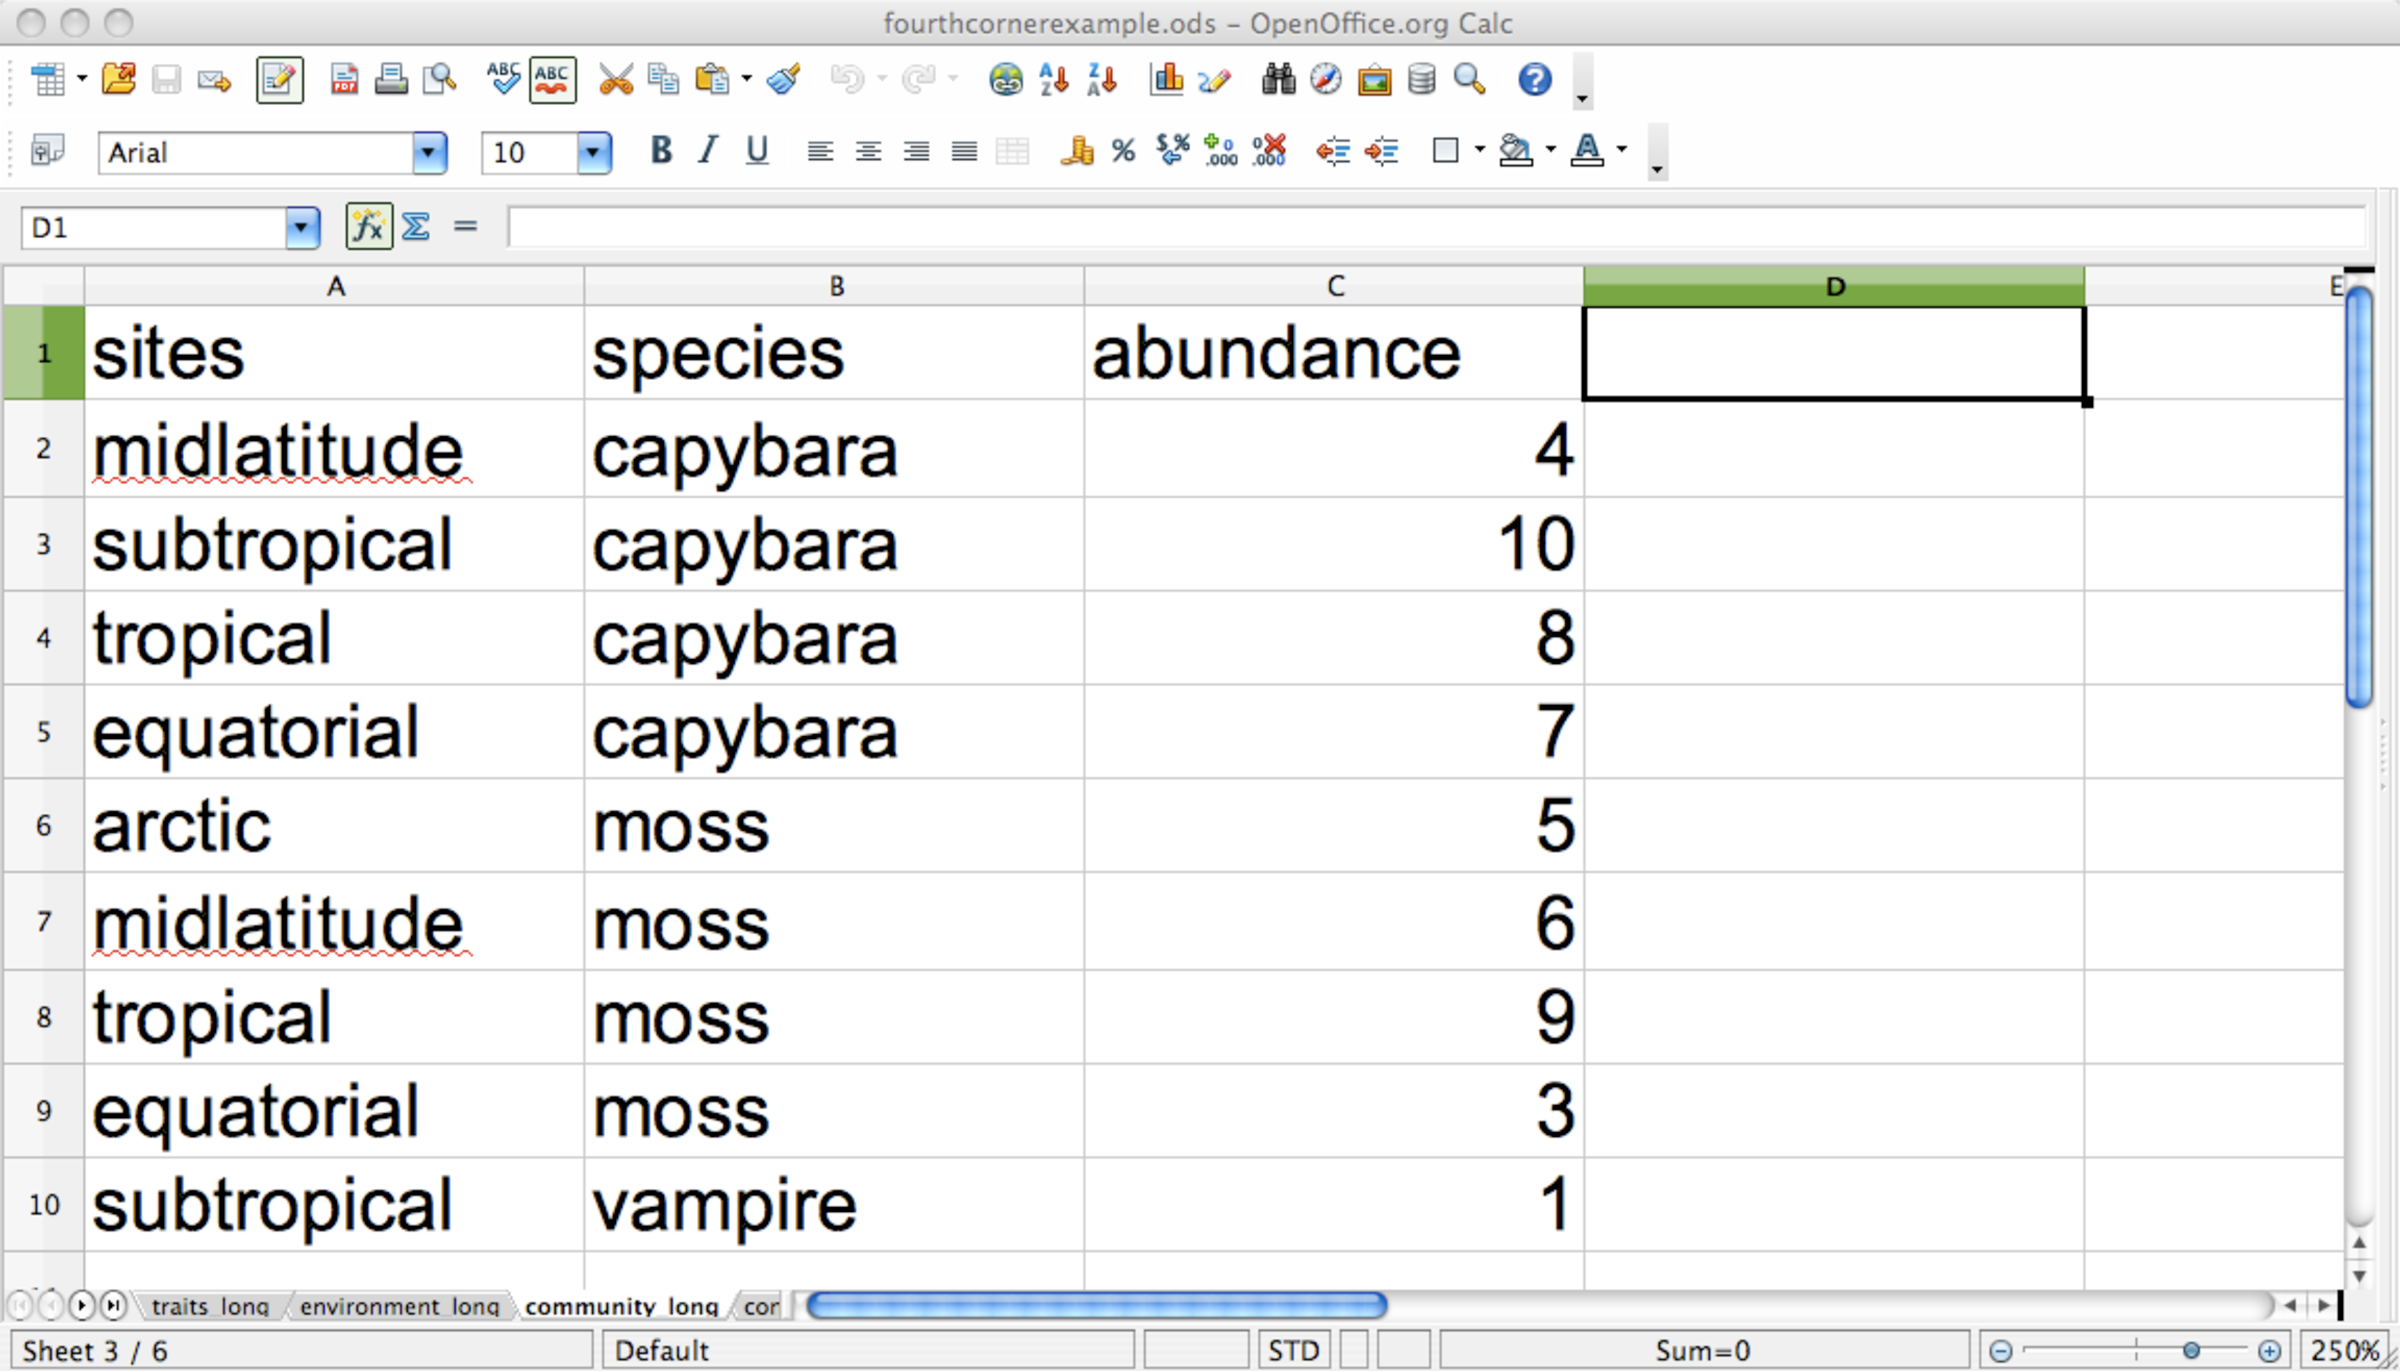
\includegraphics{./readingmultipletables/community_long.pdf}
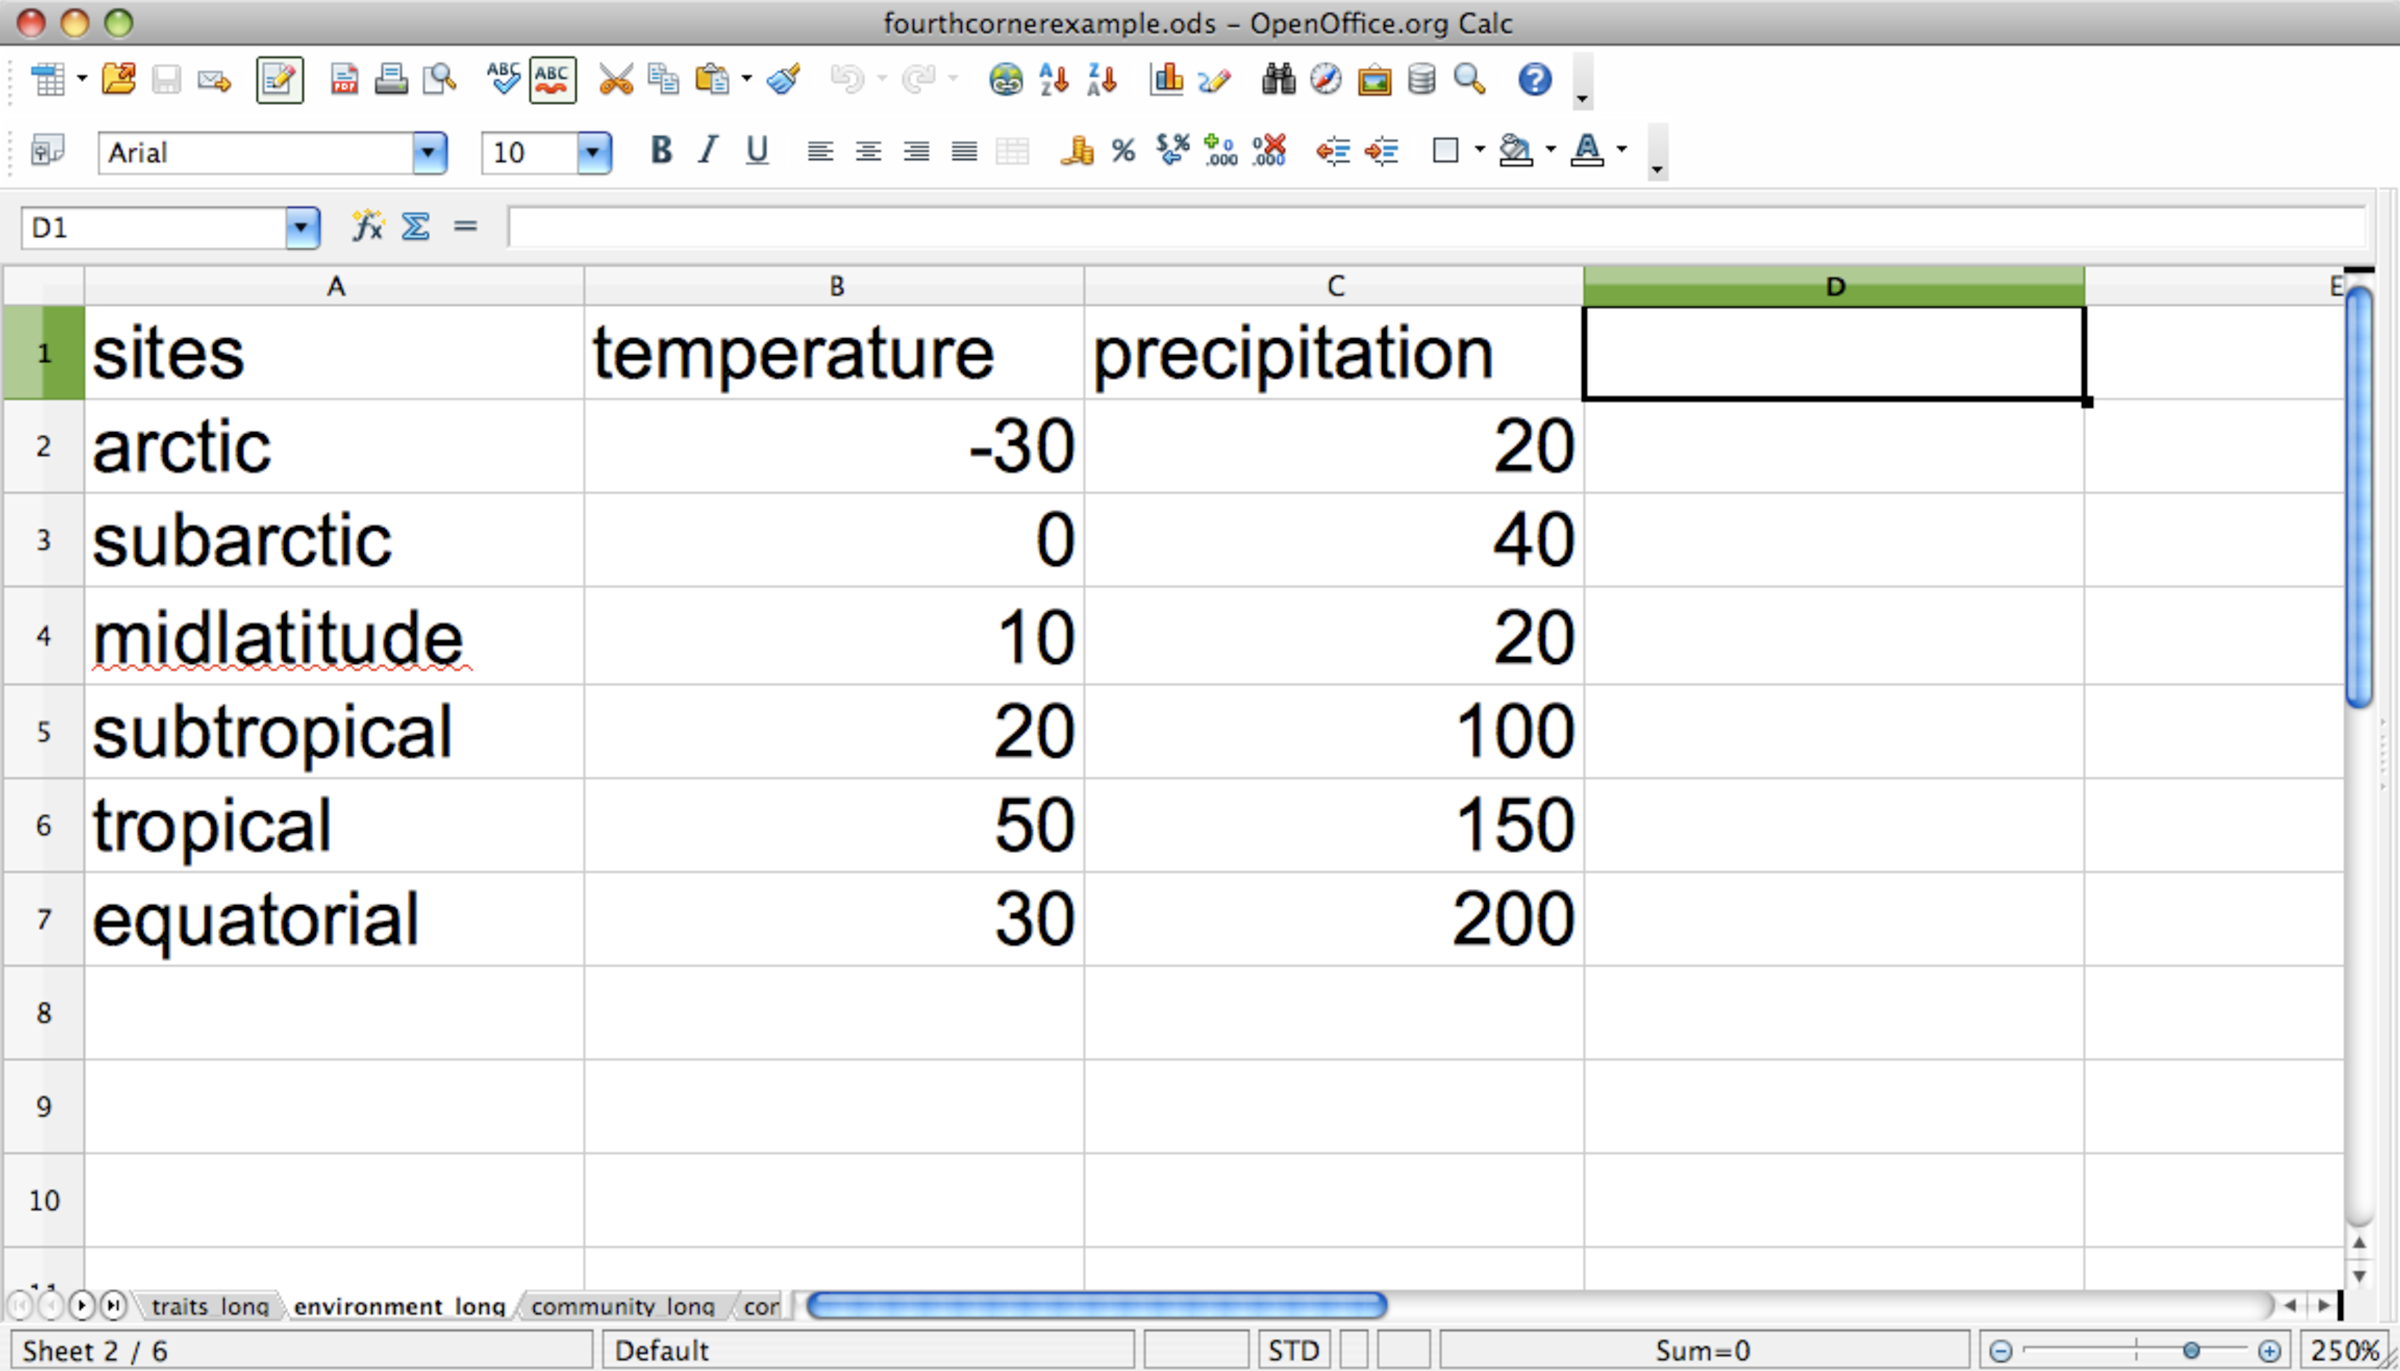
\includegraphics{./readingmultipletables/environment_long.pdf}
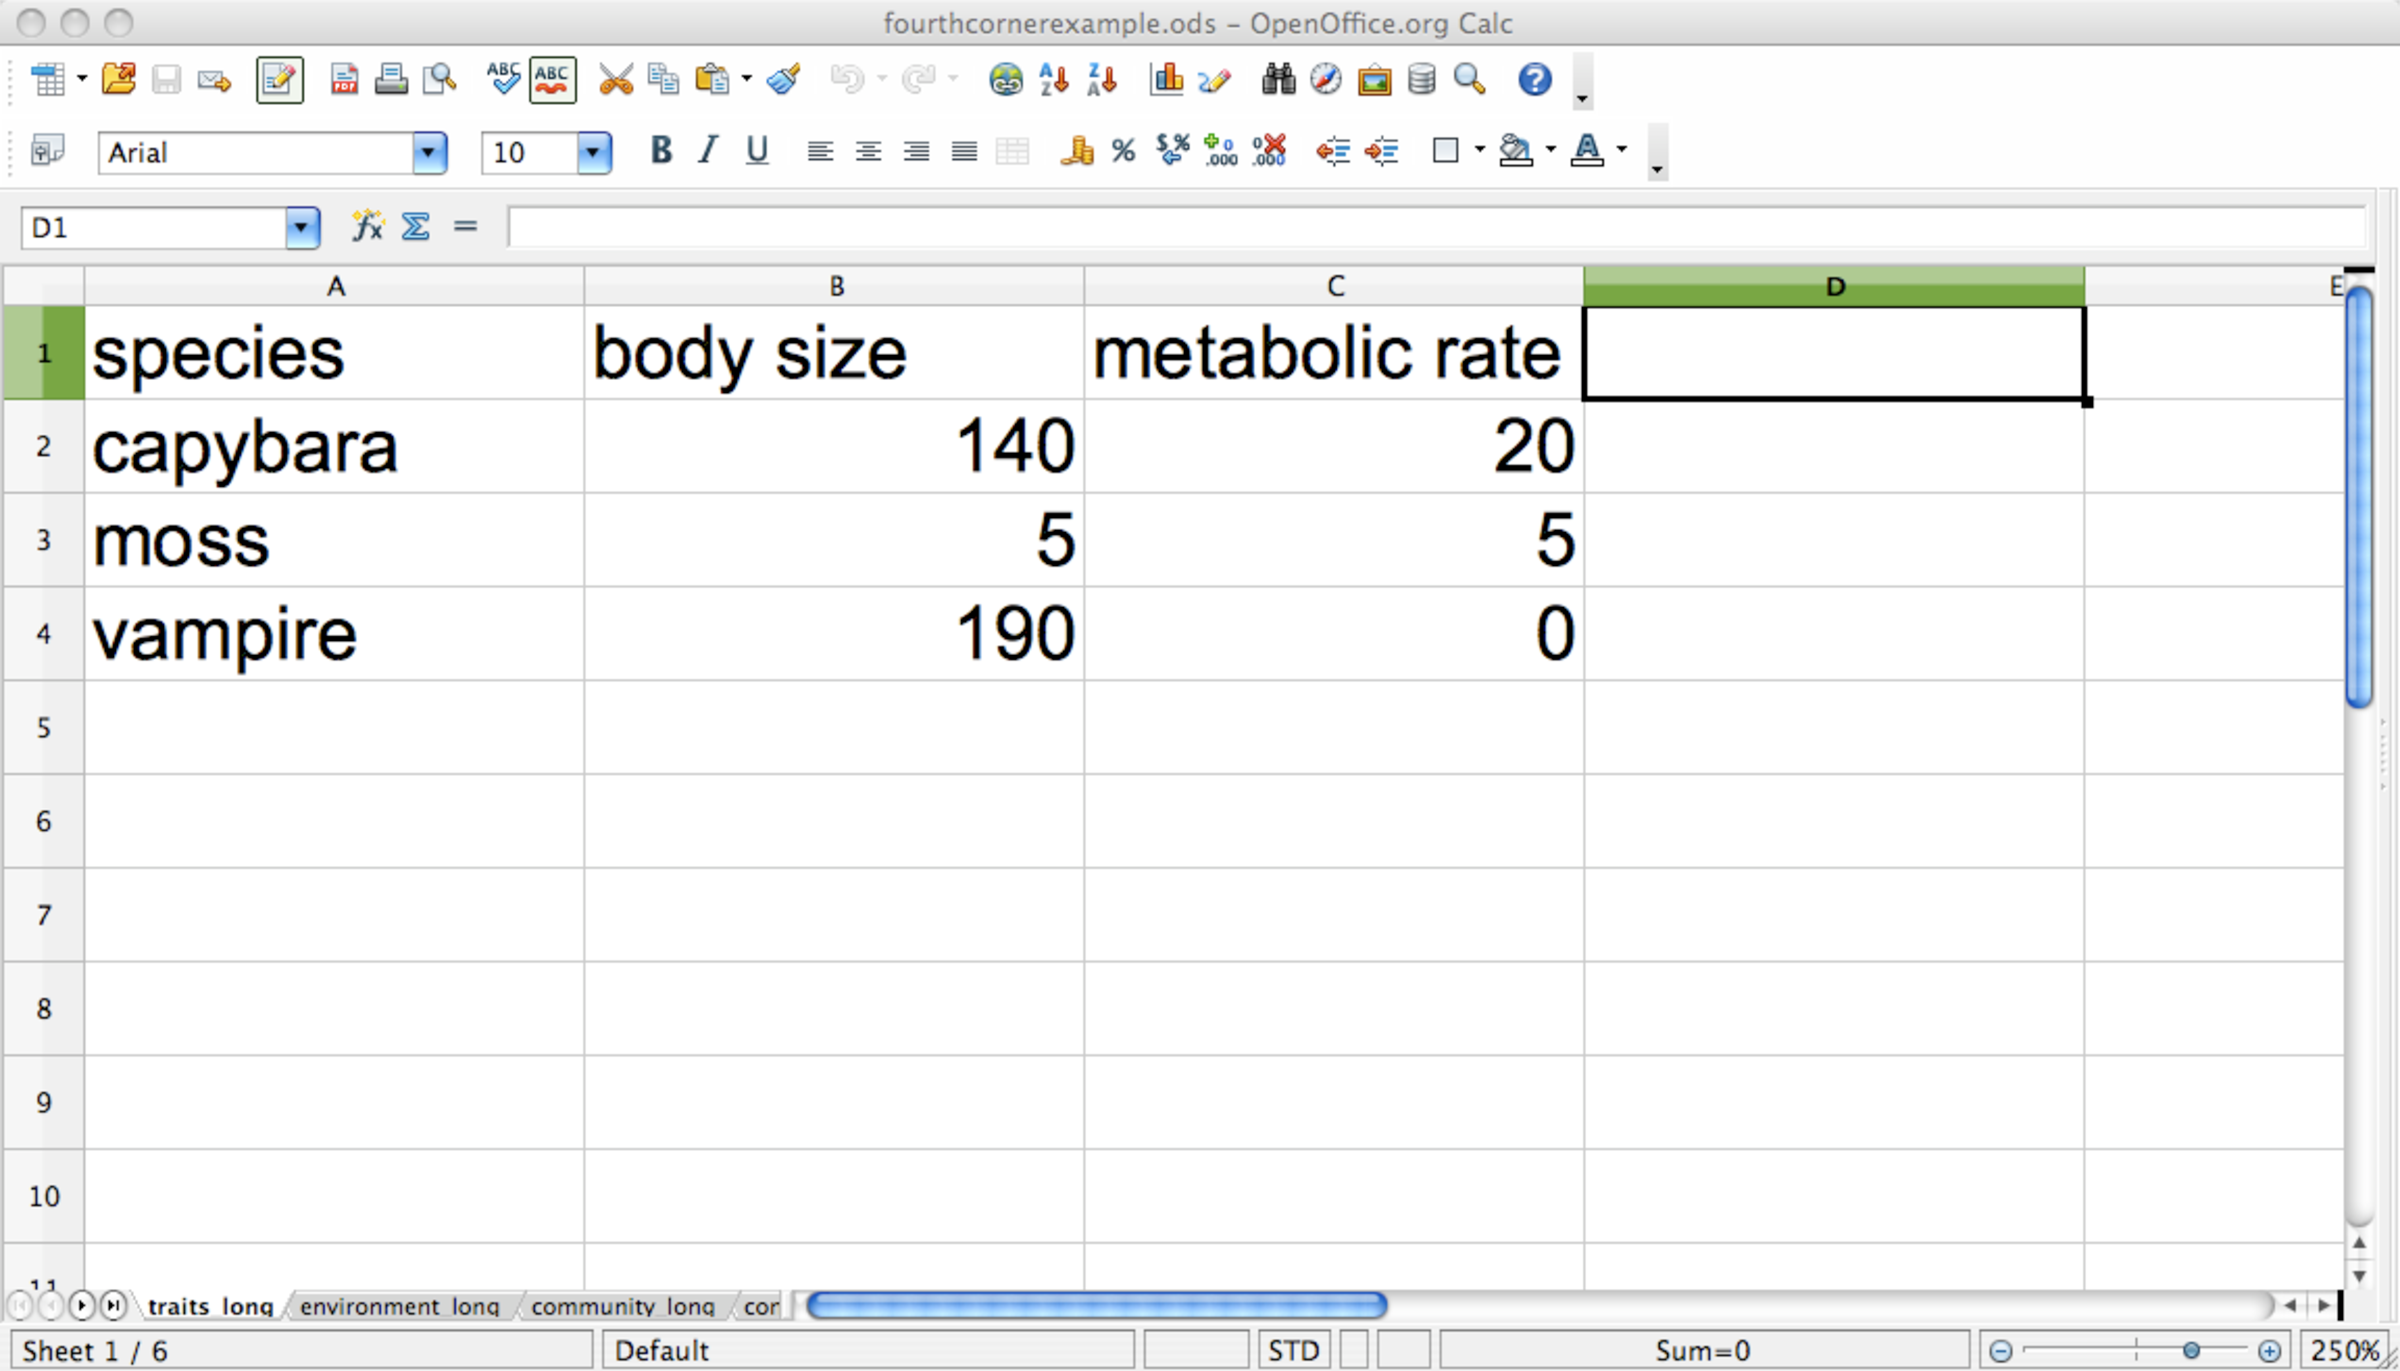
\includegraphics{./readingmultipletables/traits_long.pdf}
\caption{Fictitious fourth-corner data set in `long' format.}
\label{fig:longspreadsheetfc}
\end{figure}In this format, the community data becomes a single column (i.e. abundance).  The site and species that correspond to each abundance is identified by two additional columns (i.e. sites; species).  Notice that none of the zeros are stored, because it is implied that a species was not detected at a site if that site-species combination is not present in the long-format data.

The benefits of the long format are not just to save memory, which currently may seem quite unimportant given the size of contemporary storage devices.  However, there are other more important benefits.  Notice that in long format (Fig. \ref{fig:longspreadsheetfc}), the environment and traits matrix are almost identical as before (Fig. \ref{fig:spreadsheetfc}), except that the sites and species columns now have headings.  These headings specify how the tables are related.  Specifically, the abundance variable is replicated along both sites and species, temperature and precipitation are replicated along sites only, whereas body size and metabolic rate are replicated along species only.  Hence, the long format enjoys a certain conceptual simplicity:  each column denotes either a variable or a dimension of replication.  Such a format has the desirable property that additional sampling will add more rows, but never any columns.  Database management is much easier for such formats (refs?).  In contrast, the standard fourth-corner format (Fig. \ref{fig:spreadsheetfc}) will often require more columns as new sites are sampled, as a result of the species discovery process.  Furthermore, the long-format easily handles three- (or higher-) dimensional data cubes (or hyper-cubes), by simply adding additional columns for each dimension (see example ?? below); this is not possible in fourth-corner format.

To read data in long format into a \code{data.list}, we can use one of the functions from the \code{read.multitable} family of functions.  These functions are simply wrappers for the standard \code{read.table} functions in the \R\ \code{utils} package, so that these utilities can be used with multiple-table data.  Here we use \code{read.multicsv} to read in \code{.csv} versions of the data in Figure \ref{fig:longspreadsheetfc},
\begin{Schunk}
\begin{Sinput}
> files <- c("community_long.csv","environment_long.csv","traits_long.csv")
> dimids <- c("sites","species")
> fc <- read.multicsv(files,dimids,fill=c(0,NA,NA))
\end{Sinput}
\end{Schunk}
or with interactive menus,
\begin{Schunk}
\begin{Sinput}
> fc <- read.multicsv(multifile.choose(3),dimids,fill=c(0,NA,NA))
\end{Sinput}
\end{Schunk}
These commands store exactly the same \code{fc} object that we obtained before.  Note the \code{fill=c(0,NA,NA)} argument, which causes any missing site-species combinations to be filled with zeros and to fill missing environmental variables or traits with \code{NA}.

\subsection{Reading more complex multiple-table data}

Notwithstanding its small size, the above example is extremely simple; it contains only numeric data, has no missing values, and has only two dimensions of replication.  Here I provide an example (Fig. \ref{fig:complexspreadsheet}) \begin{figure}
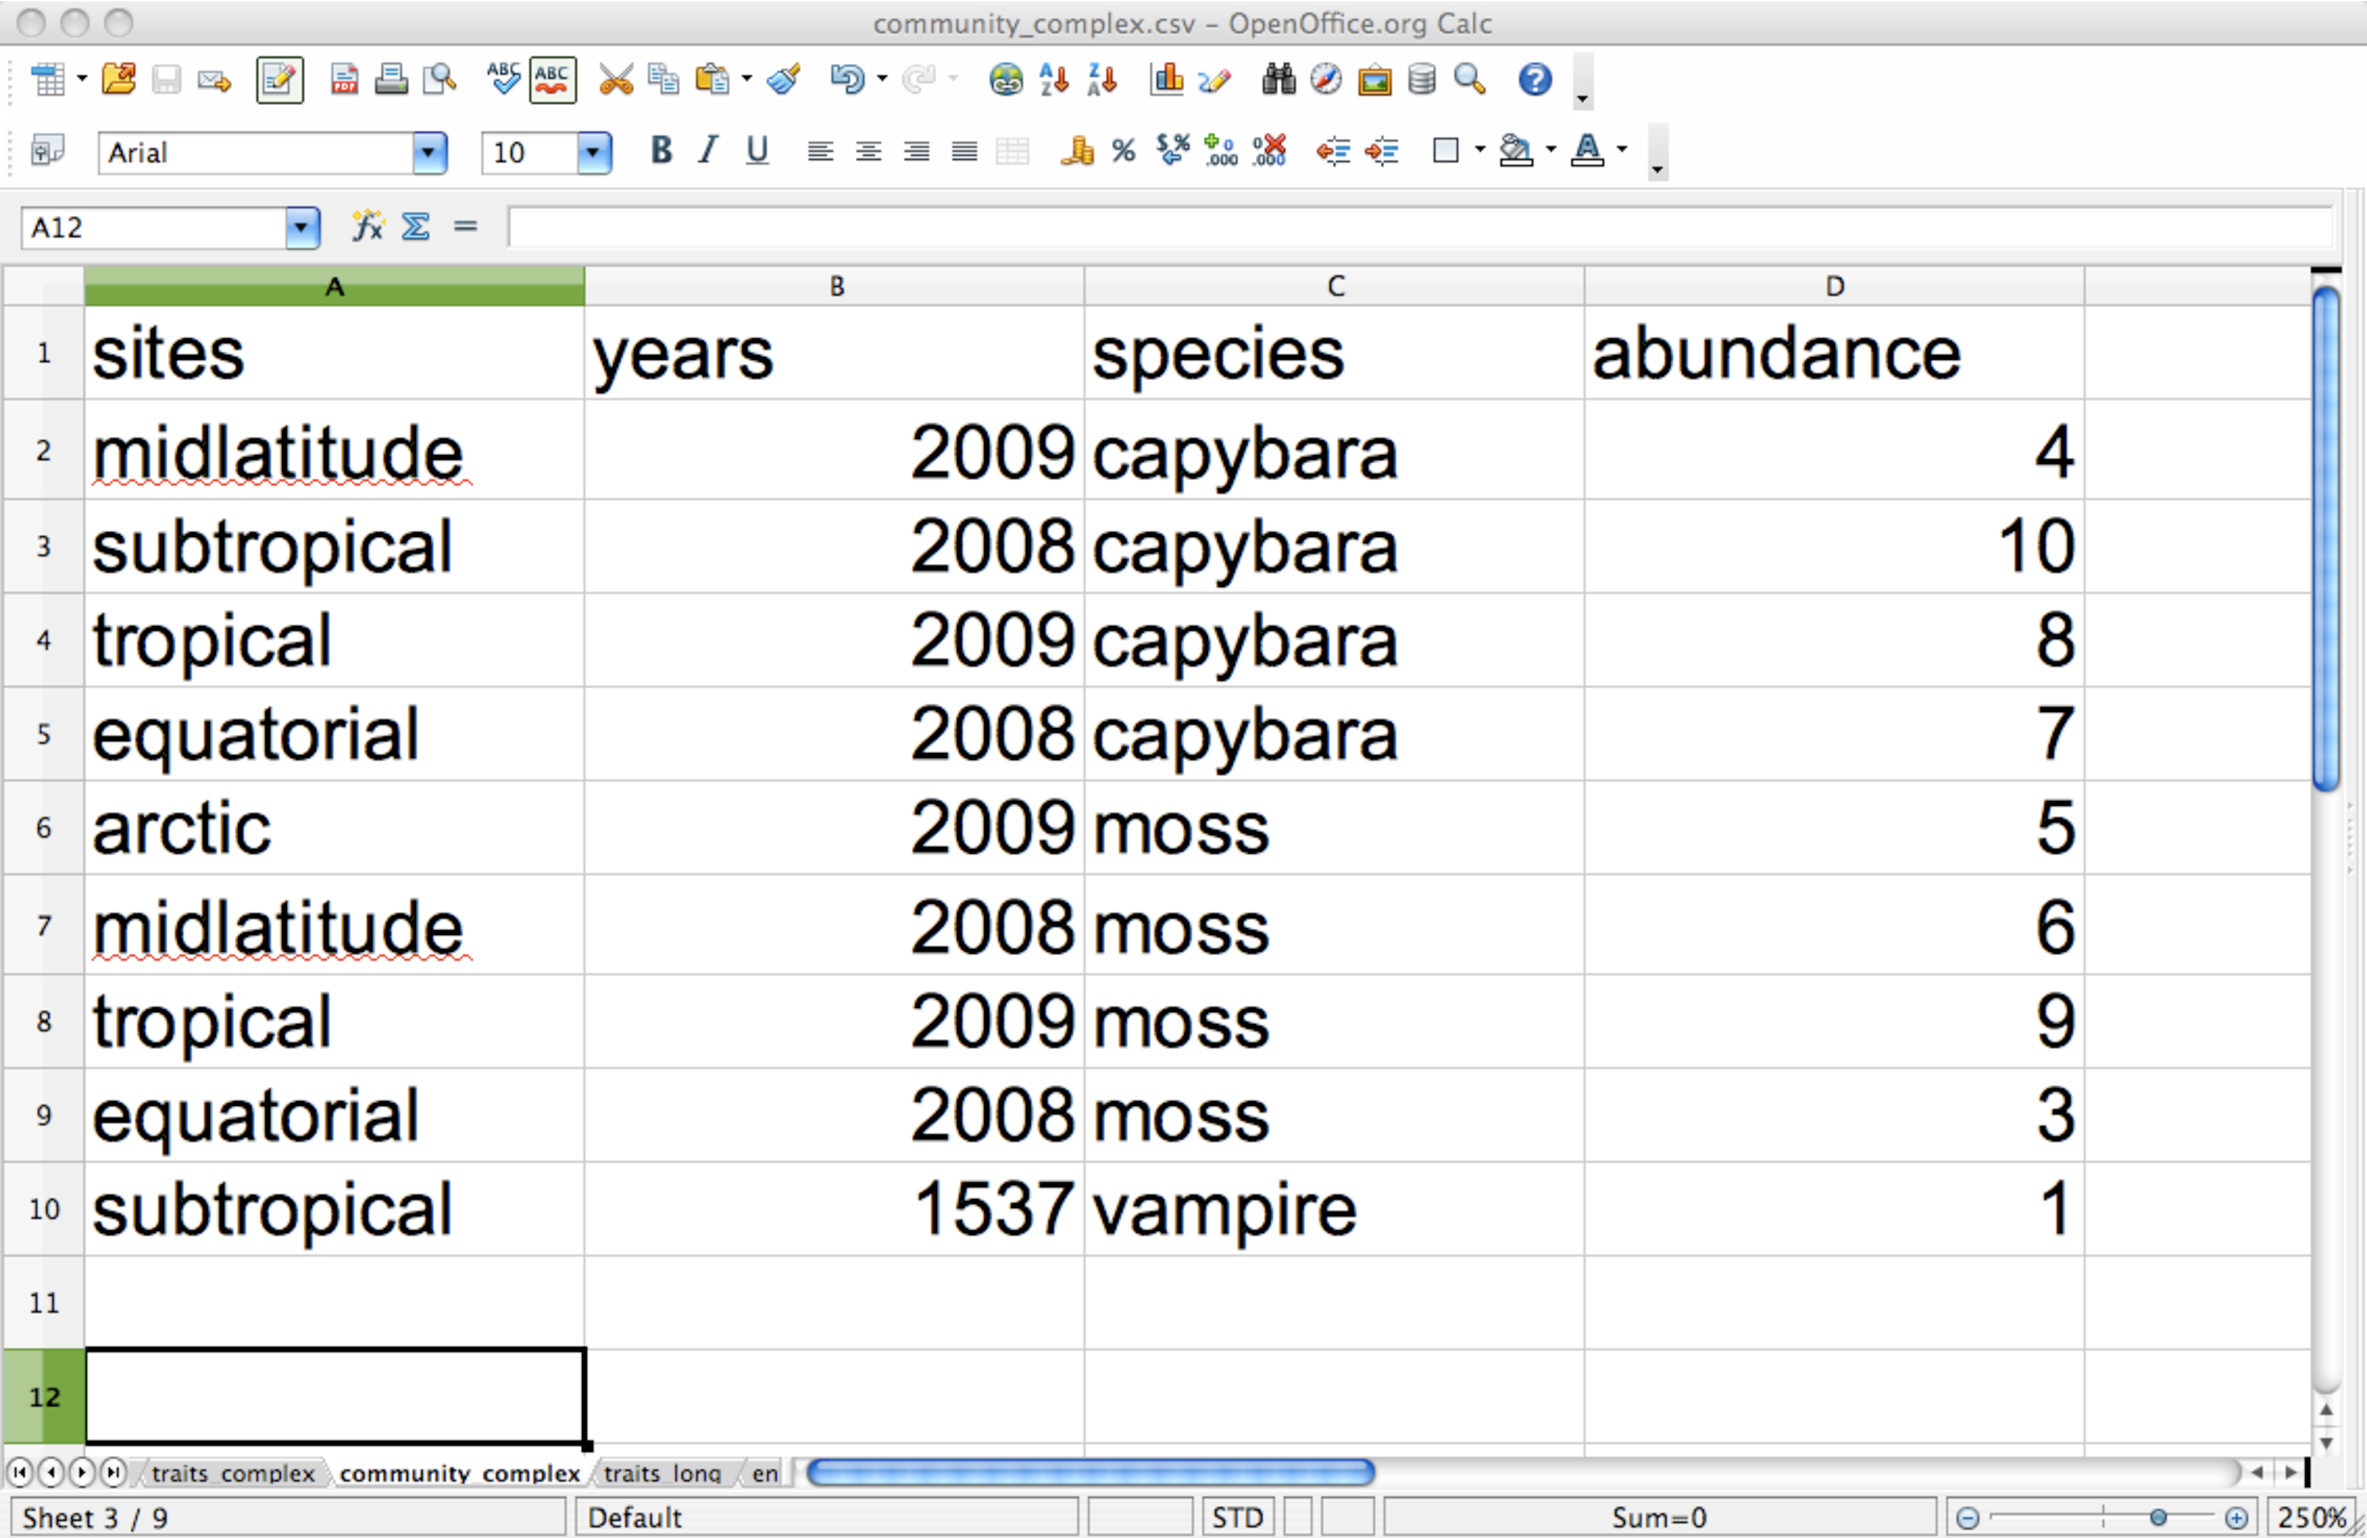
\includegraphics{./readingmultipletables/community_complex.pdf}
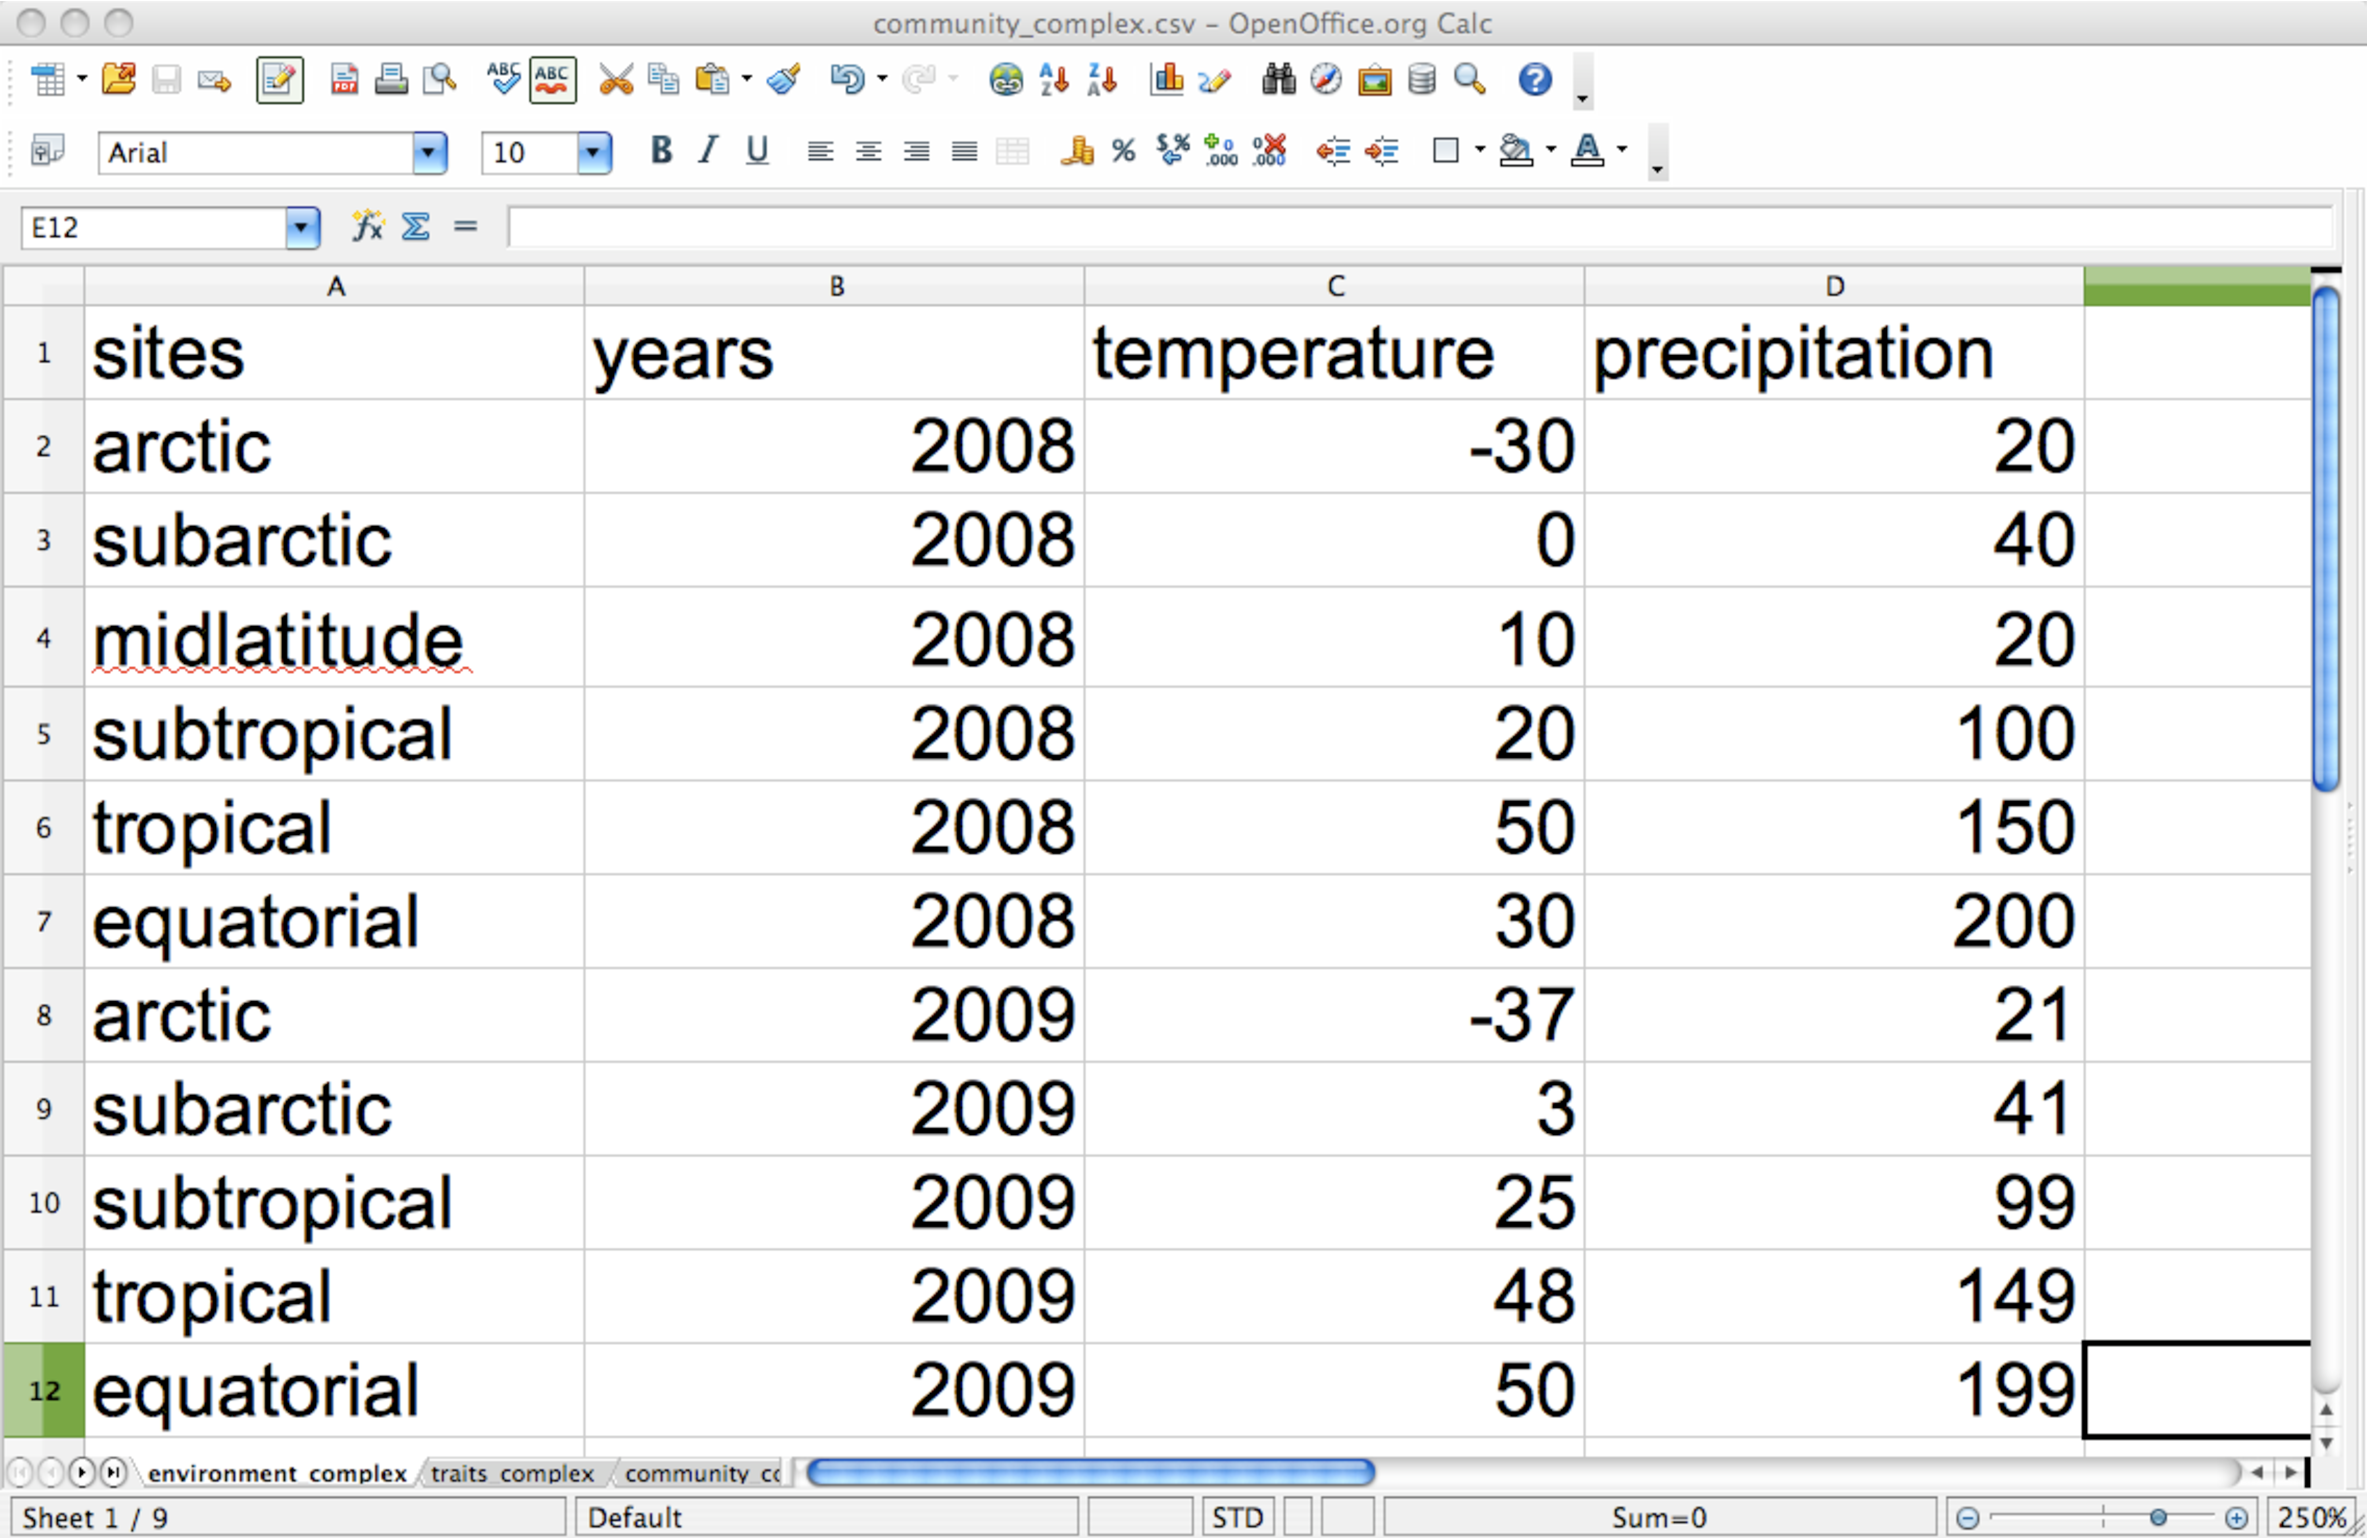
\includegraphics{./readingmultipletables/environment_complex.pdf}
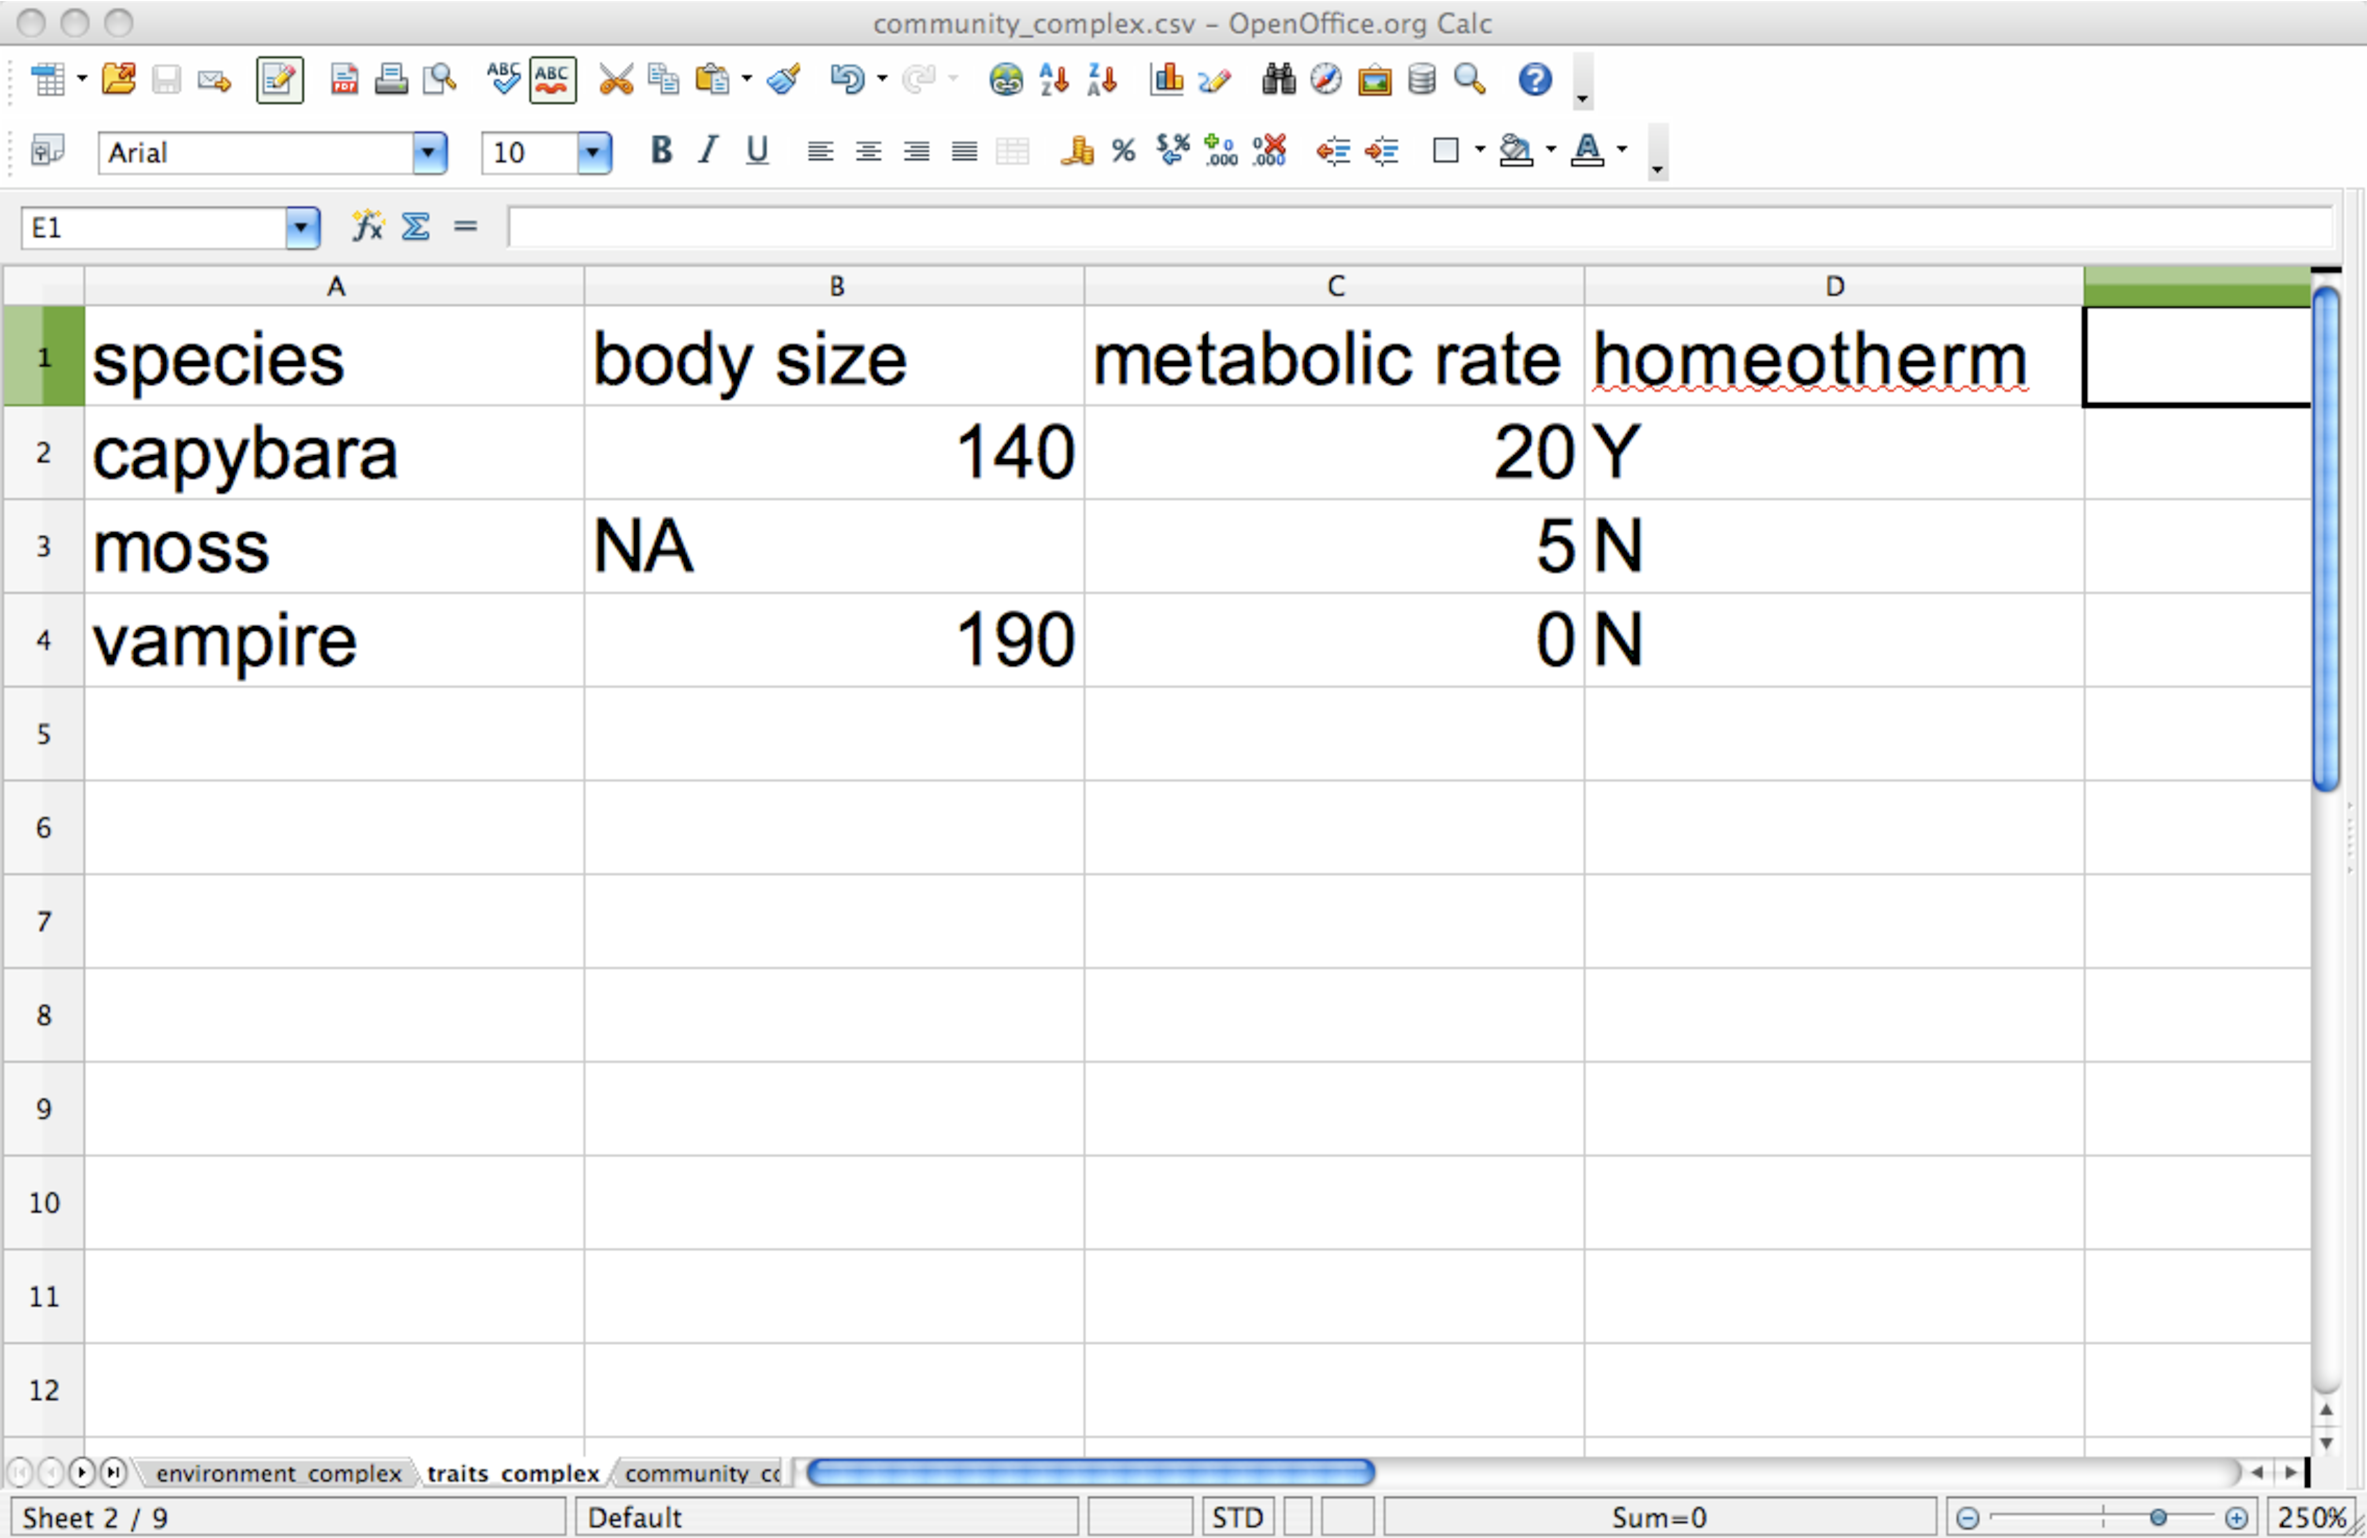
\includegraphics{./readingmultipletables/traits_complex.pdf}
\caption{Complex fictitious data set in `long' format.}
\label{fig:complexspreadsheet}
\end{figure}that relaxes those simplifications.  For the sake of space I resisted the temptation to add another file, although such an addition would pose no further difficulties.

This data set is quite a bit more complex, yet it can be read in a very similar manner to the previous data set.  The only difference is that a \code{"years"} dimension of replication must be specified.

\begin{Schunk}
\begin{Sinput}
> files <- c("community_complex.csv","environment_complex.csv","traits_complex.csv")
> dimids <- c("sites","years","species")
> fc <- read.multicsv(files,dimids,fill=c(0,NA,NA))
> fc
\end{Sinput}
\begin{Soutput}
abundance:
---------
, , capybara

            2009 2008 1537
midlatitude    4    0    0
subtropical    0   10    0
tropical       8    0    0
equatorial     0    7    0
arctic         0    0    0
subarctic      0    0    0

, , moss

            2009 2008 1537
midlatitude    0    6    0
subtropical    0    0    0
tropical       9    0    0
equatorial     0    3    0
arctic         5    0    0
subarctic      0    0    0

, , vampire

            2009 2008 1537
midlatitude    0    0    0
subtropical    0    0    1
tropical       0    0    0
equatorial     0    0    0
arctic         0    0    0
subarctic      0    0    0

Replicated along:  || sites || years || species || 


temperature:
-----------
            2009 2008 1537
midlatitude   NA   10   NA
subtropical   25   20   NA
tropical      48   50   NA
equatorial    50   30   NA
arctic       -37  -30   NA
subarctic      3    0   NA
Replicated along:  || sites || years || 


precipitation:
-------------
            2009 2008 1537
midlatitude   NA   20   NA
subtropical   99  100   NA
tropical     149  150   NA
equatorial   199  200   NA
arctic        21   20   NA
subarctic     41   40   NA
Replicated along:  || sites || years || 


body.size:
---------
capybara     moss  vampire 
     140       NA      190 
Replicated along:  || species || 


metabolic.rate:
--------------
capybara     moss  vampire 
      20        5        0 
Replicated along:  || species || 


homeotherm:
----------
capybara     moss  vampire 
       Y        N        N 
Levels: N Y
Replicated along:  || species || 


REPLICATION DIMENSIONS: 
  sites   years species 
      6       3       3 
\end{Soutput}
\end{Schunk}

\section{Creating \code{data.list} objects by combining existing \R\ objects}

So far we have covered the use of convenience functions (e.g. \code{read.multicsv}; \code{read.fourthcorner}) for directly converting multiple-table data into a \code{data.list} object.  However, experienced \R\ users will already be good at getting their data into \R\ and many such users may not wish to use our new functions, as how best to read data into \R\ is arguably a subjective matter.  Here we describe how to create \code{data.list}s from several objects (e.g. vectors; matrices; arrays; data frames; lists) that are already in \R, highlighting cases that could cause difficulties.

\subsection{Combining fourth-corner data}


Consider the following three data frames each containing part of our first data set,

\begin{Schunk}
\begin{Sinput}
> community
\end{Sinput}
\begin{Soutput}
            capybara moss vampire
arctic             0    5       0
subarctic          0    0       0
midlatitude        4    6       0
subtropical       10    0       1
tropical           8    9       0
equatorial         7    3       0
\end{Soutput}
\begin{Sinput}
> environment
\end{Sinput}
\begin{Soutput}
            temperature precipitation
arctic              -30            20
subarctic             0            40
midlatitude          10            20
subtropical          20           100
tropical             50           150
equatorial           30           200
\end{Soutput}
\begin{Sinput}
> traits
\end{Sinput}
\begin{Soutput}
         body.size metabolic.rate
capybara       140             20
moss             5              5
vampire        190              0
\end{Soutput}
\end{Schunk}

We begin with a potentially frustrating issue that could arise, and then describe its solution.  The \code{multitable} package contains a \code{data.list} function for combining multiple \R\ objects into a data list.  This function is analogous to the \code{data.frame} in the \R\ \code{base} package.  However, if we try to pass these three objects to \code{data.list}, we will get an error,
\begin{Schunk}
\begin{Sinput}
> data.list(community,environment,traits,dimids=c("sites","species"))
\end{Sinput}
\end{Schunk}
\begin{Schunk}
\begin{Soutput}
Error in check.dims(x, bm, repdim) : incompatible dimensions in body.size
\end{Soutput}
\end{Schunk}

Why didn't this work?  Well, the quick answer is that data lists must contain at least one variable that is replicated along all the dimensions of replication used by all other variables (see vignette on ????).  But why did our code result in a data list without a variable that is replicated along all dimensions (i.e. along both sites and species)?  The answer is important for understanding multiple-table data in \R, and has to do with the differences between data frames and matrices.  In standard \R\ workflows we usually don't need to worry about these differences, because many functions have the ability to work equally well with either a matrix or a data frame.  But this approach will not work with multiple-table data, because \code{data.list} will treat matrices and data frames very differently even though they look very similar.

So what's the difference between matrices and data frames?  In technical terms, a matrix is an atomic vector with a dimension attribute whereas a data frame is a list of atomic vectors without a dimension attribute.  In less technical terms, a matrix is one single variable that has been replicated along two dimensions (represented by the rows and the columns); on the other hand, a data frame is a group of several variables (represented by the columns) that has been replicated along a single dimension (represented by the rows).  The reason why this technicality is important in practice is that the structure provided by data lists is based on a distinction between dimensions of replication and groups of variables.  When a matrix is passed to \code{data.list} it `thinks' its getting one single variable that has been replicated along two dimensions, but when it gets a data frame it `thinks' its getting several variables that have only been replicated along a single dimension.

So which of our three tables should be matrices and which should be data frames?  The \code{environment} and \code{traits} tables should remain as data frames because temperature, precipitation, body size, and metabolic rate are each different variables replicated along either sites or species.  The \code{community} table should be a matrix because it is a single variable (i.e. abundance), which is replicated along both sites and species.  The error message of the previous code now makes sense.  Because we entered each of our tables as data frames, we implied that all variables were only replicated along a single dimension:  species abundances and environmental variables were replicated along sites whereas traits were replicated along species.  Therefore, none of our variables were replicated along both dimensions (i.e. sites and species), making it impossible to relate the tables.

By coercing the community data to a matrix, we can create exactly the same data list object that we obtained above for these data.
\begin{Schunk}
\begin{Sinput}
> abundance <- as.matrix(community)
> dl <- data.list(abundance,environment,traits,dimids=c("sites","species"))
\end{Sinput}
\end{Schunk}

\subsection{Combining fourth-corner data in `long' data frames}

Now suppose that the data objects are in `long' format,


\begin{Schunk}
\begin{Sinput}
> community
\end{Sinput}
\begin{Soutput}
        sites  species abundance
1 midlatitude capybara         4
2 subtropical capybara        10
3    tropical capybara         8
4  equatorial capybara         7
5      arctic     moss         5
6 midlatitude     moss         6
7    tropical     moss         9
8  equatorial     moss         3
9 subtropical  vampire         1
\end{Soutput}
\begin{Sinput}
> environment
\end{Sinput}
\begin{Soutput}
        sites temperature precipitation
1      arctic         -30            20
2   subarctic           0            40
3 midlatitude          10            20
4 subtropical          20           100
5    tropical          50           150
6  equatorial          30           200
\end{Soutput}
\begin{Sinput}
> traits
\end{Sinput}
\begin{Soutput}
   species body.size metabolic.rate
1 capybara       140             20
2     moss         5              5
3  vampire       190              0
\end{Soutput}
\end{Schunk}

We can use the \code{dlcast} function to combine these tables into a data list.  The following code will again produce an identical data list,
\begin{Schunk}
\begin{Sinput}
> dl <- dlcast(
   list(community,environment,traits),
   dimids=c("sites","species"),fill=c(0,NA,NA))
\end{Sinput}
\end{Schunk}
The \code{dlcast} function is inspired by the \code{acast} function from the \code{reshape2} package.  The \code{acast} function converts a long-format data frame into an array depending on which variables are identified as defining the dimensions of the resulting array and which variable is used to fill it.  

\subsection{Explicit specification of dimension sharing}

The \code{data.list} function uses an algorithm to identify the structure (i.e. pattern of dimension sharing) in the data objects that are being combined into a data list.  In my experience, this algorithm has worked very well.  Occasionally however, it will be unable to figure out the structure of your data, and will give an error message.  In such cases, the \code{match.dimids} argument will need to be specified, in order to explicitly pass the structure of the data to \code{data.list}.  This \code{match.dimids} argument stands for `\emph{match} the replication \emph{dim}ension \emph{id}entifier\emph{s}'.

For example, consider the following three objects.
\begin{Schunk}
\begin{Sinput}
> A <- matrix(letters[sample(1:3,9,replace=TRUE)],3,3)
> B <- runif(3)
> C <- runif(3)
> A
\end{Sinput}
\begin{Soutput}
     [,1] [,2] [,3]
[1,] "b"  "b"  "b" 
[2,] "b"  "c"  "c" 
[3,] "c"  "b"  "b" 
\end{Soutput}
\begin{Sinput}
> B
\end{Sinput}
\begin{Soutput}
[1] 0.1699835 0.5148565 0.2964128
\end{Soutput}
\begin{Sinput}
> C
\end{Sinput}
\begin{Soutput}
[1] 0.59257387 0.05096413 0.09850842
\end{Soutput}
\end{Schunk}
If we try to combine them into a data list using \code{data.list} without a \code{match.dimids} argument, we will get an error.
\begin{Schunk}
\begin{Sinput}
> data.list(A,B,C)
\end{Sinput}
\end{Schunk}
\begin{Schunk}
\begin{Soutput}
Error in make.match.dimids(x, dimids) : 
  Some dimensions are unnamed and some are 
of the same length and therefore require
specification of match.dimids. Type
?data.list and see the details section
of the help file for data.list.
\end{Soutput}
\end{Schunk}
The error message tells us that two things have gone wrong.  First, the dimensions of the objects are unnamed.  Therefore, the algorithm in \code{data.list} has received no explicit information about which dimensions are shared because it has no \code{dimnames} to compare.  Second, because all of the dimensions are of length three, it has no way of figuring out which dimensions must be shared.  For example, is the only dimension of variable \code{B} related with the first or the second dimension of variable \code{A}?  Now if one of the dimensions had length three and other length two, then everything would be fine as in the following example.
\begin{Schunk}
\begin{Sinput}
> a <- matrix(letters[sample(1:3,6,replace=TRUE)],3,2)
> b <- runif(3)
> c <- runif(2)
> data.list(a,b,c)
\end{Sinput}
\begin{Soutput}
a:
-
  1 2
1 a c
2 b b
3 a c
Levels: a b c
Replicated along:  || D1 || D2 || 


b:
-
        1         2         3 
0.4510398 0.1706515 0.3199520 
Replicated along:  || D1 || 


c:
-
        1         2 
0.5817590 0.3162734 
Replicated along:  || D2 || 


REPLICATION DIMENSIONS: 
D1 D2 
 3  2 
\end{Soutput}
\end{Schunk}
In this example, \code{b} must be related to the first dimension of \code{a} because they are both of length three, and \code{c} must be related to the second dimension of \code{a} because they are both of length two.  But in our previous example there was an ambiguity caused by the fact that both dimensions had the same length, and because no \code{dimnames} were supplied.  In such cases, we must explicitly specify which replication dimensions are related to which others using \code{match.dimids}.
\begin{Schunk}
\begin{Sinput}
> data.list(A,B,C,match.dimids=list(c("D1","D2"),"D1","D2"))
\end{Sinput}
\begin{Soutput}
A:
-
  1 2 3
1 b b b
2 b c c
3 c b b
Levels: b c
Replicated along:  || D1 || D2 || 


B:
-
        1         2         3 
0.1699835 0.5148565 0.2964128 
Replicated along:  || D1 || 


C:
-
         1          2          3 
0.59257387 0.05096413 0.09850842 
Replicated along:  || D2 || 


REPLICATION DIMENSIONS: 
D1 D2 
 3  3 
\end{Soutput}
\end{Schunk}

\bibliographystyle{ecology}
%% ***   Set the bibliography file.   ***
%% ("thesis.bib" by default; change if needed)
\bibliography{/Users/stevenwalker/Documents/Bibliography/Bibliography}

\end{document}
